%%% Presentation slides
\newcommand{\slidesfinal}{
  \documentclass[handout,style=authortitle]{beamer}
}

%%% Ignore images --- slightly faster compilation
\newcommand{\slidestest}{
  \documentclass[demo,handout,style=authortitle]{beamer}
}

%%% Printable slides with side notes thing
\newcommand{\makehandouts}{
  \usepackage{handoutWithNotes}
  \usepackage{pgfpages}
  \pgfpagesuselayout{3 on 1 with notes big}[a4paper,border shrink=7mm]
  \pgfpageslogicalpageoptions{1}{border code=\pgfusepath{stroke}}
  \pgfpageslogicalpageoptions{2}{border code=\pgfusepath{stroke}}
  \pgfpageslogicalpageoptions{3}{border code=\pgfusepath{stroke}}
}
%%% Presentation slides
\renewcommand{\slidesfinal}{
  \documentclass[handout,style=authortitle,aspectratio=43]{beamer}
}
\slidesfinal
% \slidestest
% \makehandouts

%%% Styles and settings
% -------------------------------------------------------------------------
% Author, title, etc.
% -------------------------------------------------------------------------

% author
\makeatletter
\newcommand\myshortauthor[1]{\renewcommand\@myshortauthor{#1}}
\newcommand\@myshortauthor{}
\makeatother

\makeatletter
\newcommand\myauthor[1]{\renewcommand\@myauthor{#1}}
\newcommand\@myauthor{}
\makeatother

\makeatletter
\author[\theauthorgoeshere]{\@myauthor}
\makeatother

% url
\makeatletter
\newcommand\myurl[1]{\renewcommand\@myurl{#1}}
\newcommand\@myurl{}
\makeatother

% title
\makeatletter
\newcommand\myfulltitle[1]{\renewcommand\@myfulltitle{#1}}
\newcommand\@myfulltitle{}
\makeatother

\makeatletter
\newcommand\myabbrvtitle[1]{\renewcommand\@myabbrvtitle{#1}}
\newcommand\@myabbrvtitle{}
\makeatother

% \makeatletter
% \newcommand\mytitle[1]{\renewcommand\@mytitle{#1}}
% \newcommand\@mytitle{}
% \makeatother

% date
\makeatletter
\newcommand\mydate[1]{\renewcommand\@mydate{#1}}
\newcommand\@mydate{}
\makeatother


% maketitle
\makeatletter
\newcommand{\mytitlea}{\makebox[.45\paperwidth]%
{\@myabbrvtitle\hfill\insertframenumber/\inserttotalframenumber}}
\newcommand{\mytitleb}{\@myabbrvtitle}
\makeatother


\makeatletter
\title[\mytitleb]{\@myfulltitle}
\makeatother


\makeatletter
\date{\@mydate \\[.5cm] \titlelogos}
\makeatother

\makeatletter
\newcommand{\theauthorgoeshere}{\makebox[.45\paperwidth]{%
        \@myurl \hfill \@myshortauthor}}
\makeatother

%\documentclass{beamer}
\documentclass[handout]{beamer}

\usepackage{amsmath}
\usepackage{beamerthemesplit}
\usepackage{fancybox}
\usepackage{hyperref}
\usepackage{color}
\usepackage{listings}


\makeatletter
\newcommand\code{\bgroup\@makeother\_\@makeother\~\@makeother\$\@codex}
\def\@codex#1{{\normalfont\ttfamily\hyphenchar\font=-1 #1}\egroup}
\makeatother

\newcommand{\bX}{\boldsymbol{X}}
\newcommand{\bx}{\boldsymbol{x}}
\newcommand{\by}{\boldsymbol{y}}
\newcommand{\bbeta}{\boldsymbol{\beta}}
\newcommand{\bepsilon}{\boldsymbol{\epsilon}}
\newcommand{\bs}[1]{\boldsymbol{#1}}


\definecolor{gray}{rgb}{.6,.6,.6}
\definecolor{orange}{rgb}{1,0.5,0}
\definecolor{grayish}{rgb}{.775, .775, .775}
\definecolor{dkgray}{rgb}{.375, .375, .375}
\definecolor{dkgreen}{rgb}{0,0.6,0}
\definecolor{mauve}{rgb}{0.58,0,0.82}
\definecolor{dkblue}{rgb}{0, 0, .5}
\definecolor{purple}{rgb}{0.7, 0, 0.5}

\definecolor{g11}{rgb}{0, 0, 1}
\definecolor{g12}{rgb}{0, .4, 1}
\definecolor{g13}{rgb}{0, .8, 1}

\definecolor{g21}{rgb}{0, .5, .3}
\definecolor{g22}{rgb}{.4, .5, .3}
\definecolor{g23}{rgb}{.8, .5, .3}

\lstset{ %
  language=R,     
  numbers=left,
  stepnumber=1,       
  numbersep=6pt,      
  showspaces=false,      
  showstringspaces=false,  
  showtabs=false,    
  frame=single,      
  rulecolor=\color{black},   
  tabsize=4,     
  captionpos=t,     
  breaklines=true,     
  breakatwhitespace=true,   
  title=\lstname,              
  basicstyle=\ttfamily\color{black}\scriptsize, 
  backgroundcolor=\color{grayish},  
  numberstyle=\tiny\color{black},  
  keywordstyle=\color{blue}, 
  commentstyle=\color{dkgreen}, 
  stringstyle=\color{mauve}, 
  xleftmargin=.1in,
  xrightmargin=.1in,
  aboveskip=0cm,
  belowskip=.2cm
  %   escapeinside={\%*}{*)},    
%   morekeywords={*,...}    
}

\setbeamertemplate{navigation symbols}{} 

\hypersetup{
    linkcolor=,
    colorlinks=true,
    urlcolor=blue
}

\usetheme{Frankfurt}
% \usecolortheme{whale}
% \usetheme{Antibes}
% \setbeamertemplate{mini frames}{}


\newcommand{\fctn}[1]{\textcolor{green!50!blue}{#1}}
\newcommand{\rfor}[1]{\textcolor{yellow!50!red}{#1}}
\newcommand{\rcom}[1]{\textcolor{blue}{#1}}

\newcommand{\pkg}[1]{\textbf{#1}}

\newcommand{\startr}{\begin{minipage}{.04\textwidth}\ \ \end{minipage} \begin{minipage}{.91\textwidth}}

%
\newcommand{\shownum}{\title[\mytitlea]}{}
\newcommand{\hidenum}{\title[\mytitleb]{}}
% \expandafter\def\expandafter\insertshorttitle\expandafter{\insertshorttitle\hfill\insertframenumber\,/\,\inserttotalframenumber}
 

\newcounter{excount}
\setcounter{excount}{0}
\newcommand{\countex}{\addtocounter{excount}{1}\arabic{excount}}
\newcommand{\showex}{\arabic{excount}}






\useoutertheme{miniframes}
\makeatletter
  \beamer@compressfalse
\makeatother

\title{From 1 core to Thousands: R to pbdR}
\author[http://r-pbd.org \hspace{2.5cm}  pbdR Core]{%
  George Ostrouchov$^{1,2}$ and Drew Schmidt$^2$
%  and Wei-Chen Chen$^1$,
%  and Pragneshkumar Patel$^2$
\\[1em]
{$^1$Oak Ridge National Laboratory, Oak Ridge, TN} \\
{$^2$University of Tennessee, Knoxville, TN} \\[5em]
OLCF Workshop \\ on  Processing and Analysis of Very Large Data Sets \\
August 8, 2013}
\date{}
\logo{
  \begin{tabular}{r}
    
\includegraphics[height=.34cm]{../common/pics/ornl.jpg} \\
    
\includegraphics[height=.34cm]{../common/pics/utk_logo.png}
  \end{tabular}
}

\newcommand{\mytitlea}{Programming with Big Data in R \hspace{5em} \insertframenumber\,/\,\inserttotalframenumber}
\newcommand{\mytitleb}{Programming with Big Data in R}

%%%%%%%%%%%%%%%%%%%%%%%%%%%%%%%%%%%%%%%%%%%%%%%%%%%%%%%%%%%%%%%%%%%%%%%%%%%%%%%%%
%%%%%%%%%%%%%%%%%%%%%%%%%%%%%%%%%%%%%%%%%%%%%%%%%%%%%%%%%%%%%%%%%%%%%%%%%%%%%%%%%
%%%%%%%%%%%%%%%%%%%%%%%%%%%%%%%%%%%%%%%%%%%%%%%%%%%%%%%%%%%%%%%%%%%%%%%%%%%%%%%%%
\begin{document}

%%%%%%%%%%%%%%%%%%%%%%%%%%%%%%%%%%%%%%%%
%%     Title and ToC
%%%%%%%%%%%%%%%%%%%%%%%%%%%%%%%%%%%%%%%%
% titlepage
\frame{\maketitle}

\setcounter{footnote}{0}

\begin{frame}[noframenumbering]
\frametitle{The \pbdR\ Core Team}
\begin{minipage}{1\textwidth}
  \vspace{-.6cm}
\begin{minipage}{3.6cm}
\ \\[.8cm]
Wei-Chen Chen$^1$ \\
George Ostrouchov$^{2,3}$ \\
Pragneshkumar Patel$^3$ \\
Drew Schmidt$^3$\\[2ex]
\end{minipage}
\begin{minipage}{7cm}
  \ \hfill 
\includegraphics[width=5.5cm]{../common/pics/logos/newpbdr}
\end{minipage}
\end{minipage}
  \begin{minipage}{2.2cm}\tiny
    $^1$FDA\\
    Washington, DC, USA
  \end{minipage}
  \hspace{1ex}
  \begin{minipage}{5cm}\tiny
    $^2$Computer Science and Mathematics Division\\
    Oak Ridge National Laboratory, Oak Ridge TN, USA
  \end{minipage}
  \hspace{1ex}
  \begin{minipage}{4cm}\tiny
    $^3$Joint Institute for Computational Sciences\\
    University of Tennessee, Knoxville TN, USA
  \end{minipage}

\begin{block}{Support}\tiny
  This material is based upon work supported by the National Science
  Foundation Division of Mathematical Sciences under Grant No. 1418195.
  This work used resources of the \textcolor{blue}{National Institute for
  Computational Sciences} at the University of Tennessee, Knoxville,
  which is supported by the Office of Cyberinfrastructure of the
  U.S. National Science Foundation under Award  No. ARRA-NSF-OCI-0906324
  for NICS-RDAV center.
  This work also used resources of the \textcolor{blue}{Oak Ridge
  Leadership Computing Facility} at the Oak Ridge National
  Laboratory, which is supported by the Office of Science of the
  U.S. Department of Energy under Contract No. DE-AC05-00OR22725.\\[.2cm]
\end{block}
\end{frame}

\begin{frame}
  \frametitle{About This Presentation}
  \begin{block}{Downloads}\scriptsize
    You can update the \pbdR presentations and scripts in your virtual
    machine with: \\ \tt
    \$ cd \\
    \$ scp USERNAME@anselm.it4i.cz:/home/adios/slides/pbdr\_overview.pdf slides \\
    \$ scp
    USERNAME@anselm.it4i.cz:/home/adios/slides/pbdr\_tutorial.pdf
    slides \\
    rm -r scripts \\
    \$ scp -r USERNAME@anselm.it4i.cz:/home/adios/pbdR/scripts .
 \end{block}
\end{frame}

% \begin{frame}
% \frametitle{About This Presentation}
%   \begin{block}{Tutorial Evaluations}
%     \begin{center}
%       \url{http://bit.ly/sc13-tut-mf08}
%     \end{center}
%   \end{block}
% \end{frame}


\begin{frame}
\frametitle{About This Presentation}
 \begin{block}{Installation Instructions}
  Installation instructions for setting up a \pbdR environment are available:
  \begin{center}
  \url{http://r-pbd.org/install.html}
  \end{center}
  This includes instructions for installing R, MPI, and \pbdR.
 \end{block}
\end{frame}

% \begin{frame}%[allowframebreaks=0.8]
% \frametitle{About This Presentation}
%  \begin{block}{Conventions}
%   \begin{itemize}
%     \item We use ``{\Huge$ .$}'' as a decimal mark, not ``{\Huge$,$}''.  E.g.,
% 	``one thousand and one half'' is written ``$1,000.5$'', not ``$1.000,5$''.
%     \item We will use special suffixes to denote distributed objects (ones not
% 	stored entirely on a single processor).\\
%     \code{.spmd} denotes a distributed object, while\\
%     \code{.dmat} denotes a distributed object which is of class
% 	\code{ddmatrix}\\
%     No suffix means the object is global (common to all processors)\\[.2cm]
%     Neither of these suffices carries semantic meaning.
%     \end{itemize}
%  \end{block}
% \end{frame}



% \begin{frame}[fragile]
% \frametitle{About This Presentation}
%  \begin{block}{Conventions For Code Presentation}
% We will use two different forms of syntax highlighting.  One for displaying
% results from an interactive R session:
% \begin{lstlisting}[backgroundcolor=\color{white},basicstyle=\ttfamily\color{
% dkgray}\scriptsize,keywordstyle=\color{black},
%   commentstyle=\color{orange},stringstyle=\color{mauve}]
% R> "interactive"
% [1] "interactive"
% \end{lstlisting}
% and one for presenting R scripts
% \begin{lstlisting}
% "not interactive"
% \end{lstlisting}
%  \end{block}
% \end{frame}



\begin{frame}[noframenumbering,shrink]
\frametitle{Contents}
\small
\tableofcontents[hideallsubsections]
\end{frame}

\setcounter{framenumber}{0}
\section{Introduction}
\makesubcontentsslides


%%% Hardware slides
% \input{misc/hardware}


%%% Intro to parallelism
% \input{misc/parallelism}



\subsection{R and Parallelism}


\begin{frame}
%  \addtocounter{framenumber}{-1}
  \begin{block}{R and Parallelism}\pause
  What about R?
  \end{block}
\end{frame}

\begin{frame}
%  \addtocounter{framenumber}{-1}
  \begin{block}{Problems with Serial R}\pause
  \begin{enumerate}[<+-|alert@+>]
    \item Slow.
    \item If you don't know what you're doing, it's \emph{really} slow.
    \item Performance improvements usually for small machines.
    \item Very ram intensive.
  \end{enumerate}
  \end{block}
\end{frame}


\begin{frame}
  \begin{block}{Why We Need Parallelism}\pause
    \begin{enumerate}[<+-|alert@+>]
      \item Saves compute time.
      \item Data size is skyrocketing.
      \item Necessary for many problems.
      \item Its necessity is coming.
      \item \emph{It's really cool.}
  \end{enumerate}
  \end{block}
\end{frame}

\begin{frame}
  \begin{block}{Recall: Parallel R Packages}
   \begin{center}
    \begin{minipage}{.45\textwidth}
    \begin{block}{Shared Memory}
      \begin{enumerate}[<+-|alert@+>]
        \item \pkg{foreach}
        \item \pkg{parallel}
        \item \pkg{snow}
        \item \pkg{multicore}
      \end{enumerate}
    \end{block}
    \end{minipage}
    \hspace{.2cm}
    \begin{minipage}{.45\textwidth}
    \begin{block}{Distributed}
      \begin{enumerate}[<+-|alert@+>]
        \item \pkg{Rmpi}
        \item R+Hadoop
        \item \pkg{pbdR}
      \end{enumerate}
    \end{block}
    \end{minipage}
    \end{center}
    (and others\dots)
    \end{block}
\end{frame}



\begin{frame}[shrink]
  \begin{block}{R and Parallelism}
    The solution to many of R's problems is parallelism.  However \dots\vspace{-.4cm}
   \begin{center}
    \begin{minipage}[t]{.95\textwidth}
    \begin{block}{\centering What we have}
      \begin{enumerate}[<+-|alert@+>]
        \item Mostly serial.
        \item Mostly not distributed
        \item Data parallelism mostly explicit
      \end{enumerate}
    \end{block}
    \end{minipage}
    \\\pause
    \begin{minipage}[t]{.95\textwidth}
    \begin{block}{\centering What we want}
      \begin{enumerate}[<+-|alert@+>]
        \item Mostly parallel.
        \item Mostly distributed.
        \item Mostly implicit.
      \end{enumerate}
    \end{block}
    \end{minipage}
    \end{center}
    \end{block}
\end{frame}



\begin{frame}
  \begin{block}{R and Parallelism}
    Likewise, the HPC community is looking for high-level languages for data\dots
    \end{block}
\end{frame}


\section{pbdR}
\makesubcontentsslides

\subsection{The pbdR Project}
\makesubcontentsslidessec

\begin{frame}{\pbdR Interfaces to Libraries: Sustainable Path}
  \vspace{-1ex}
  \centering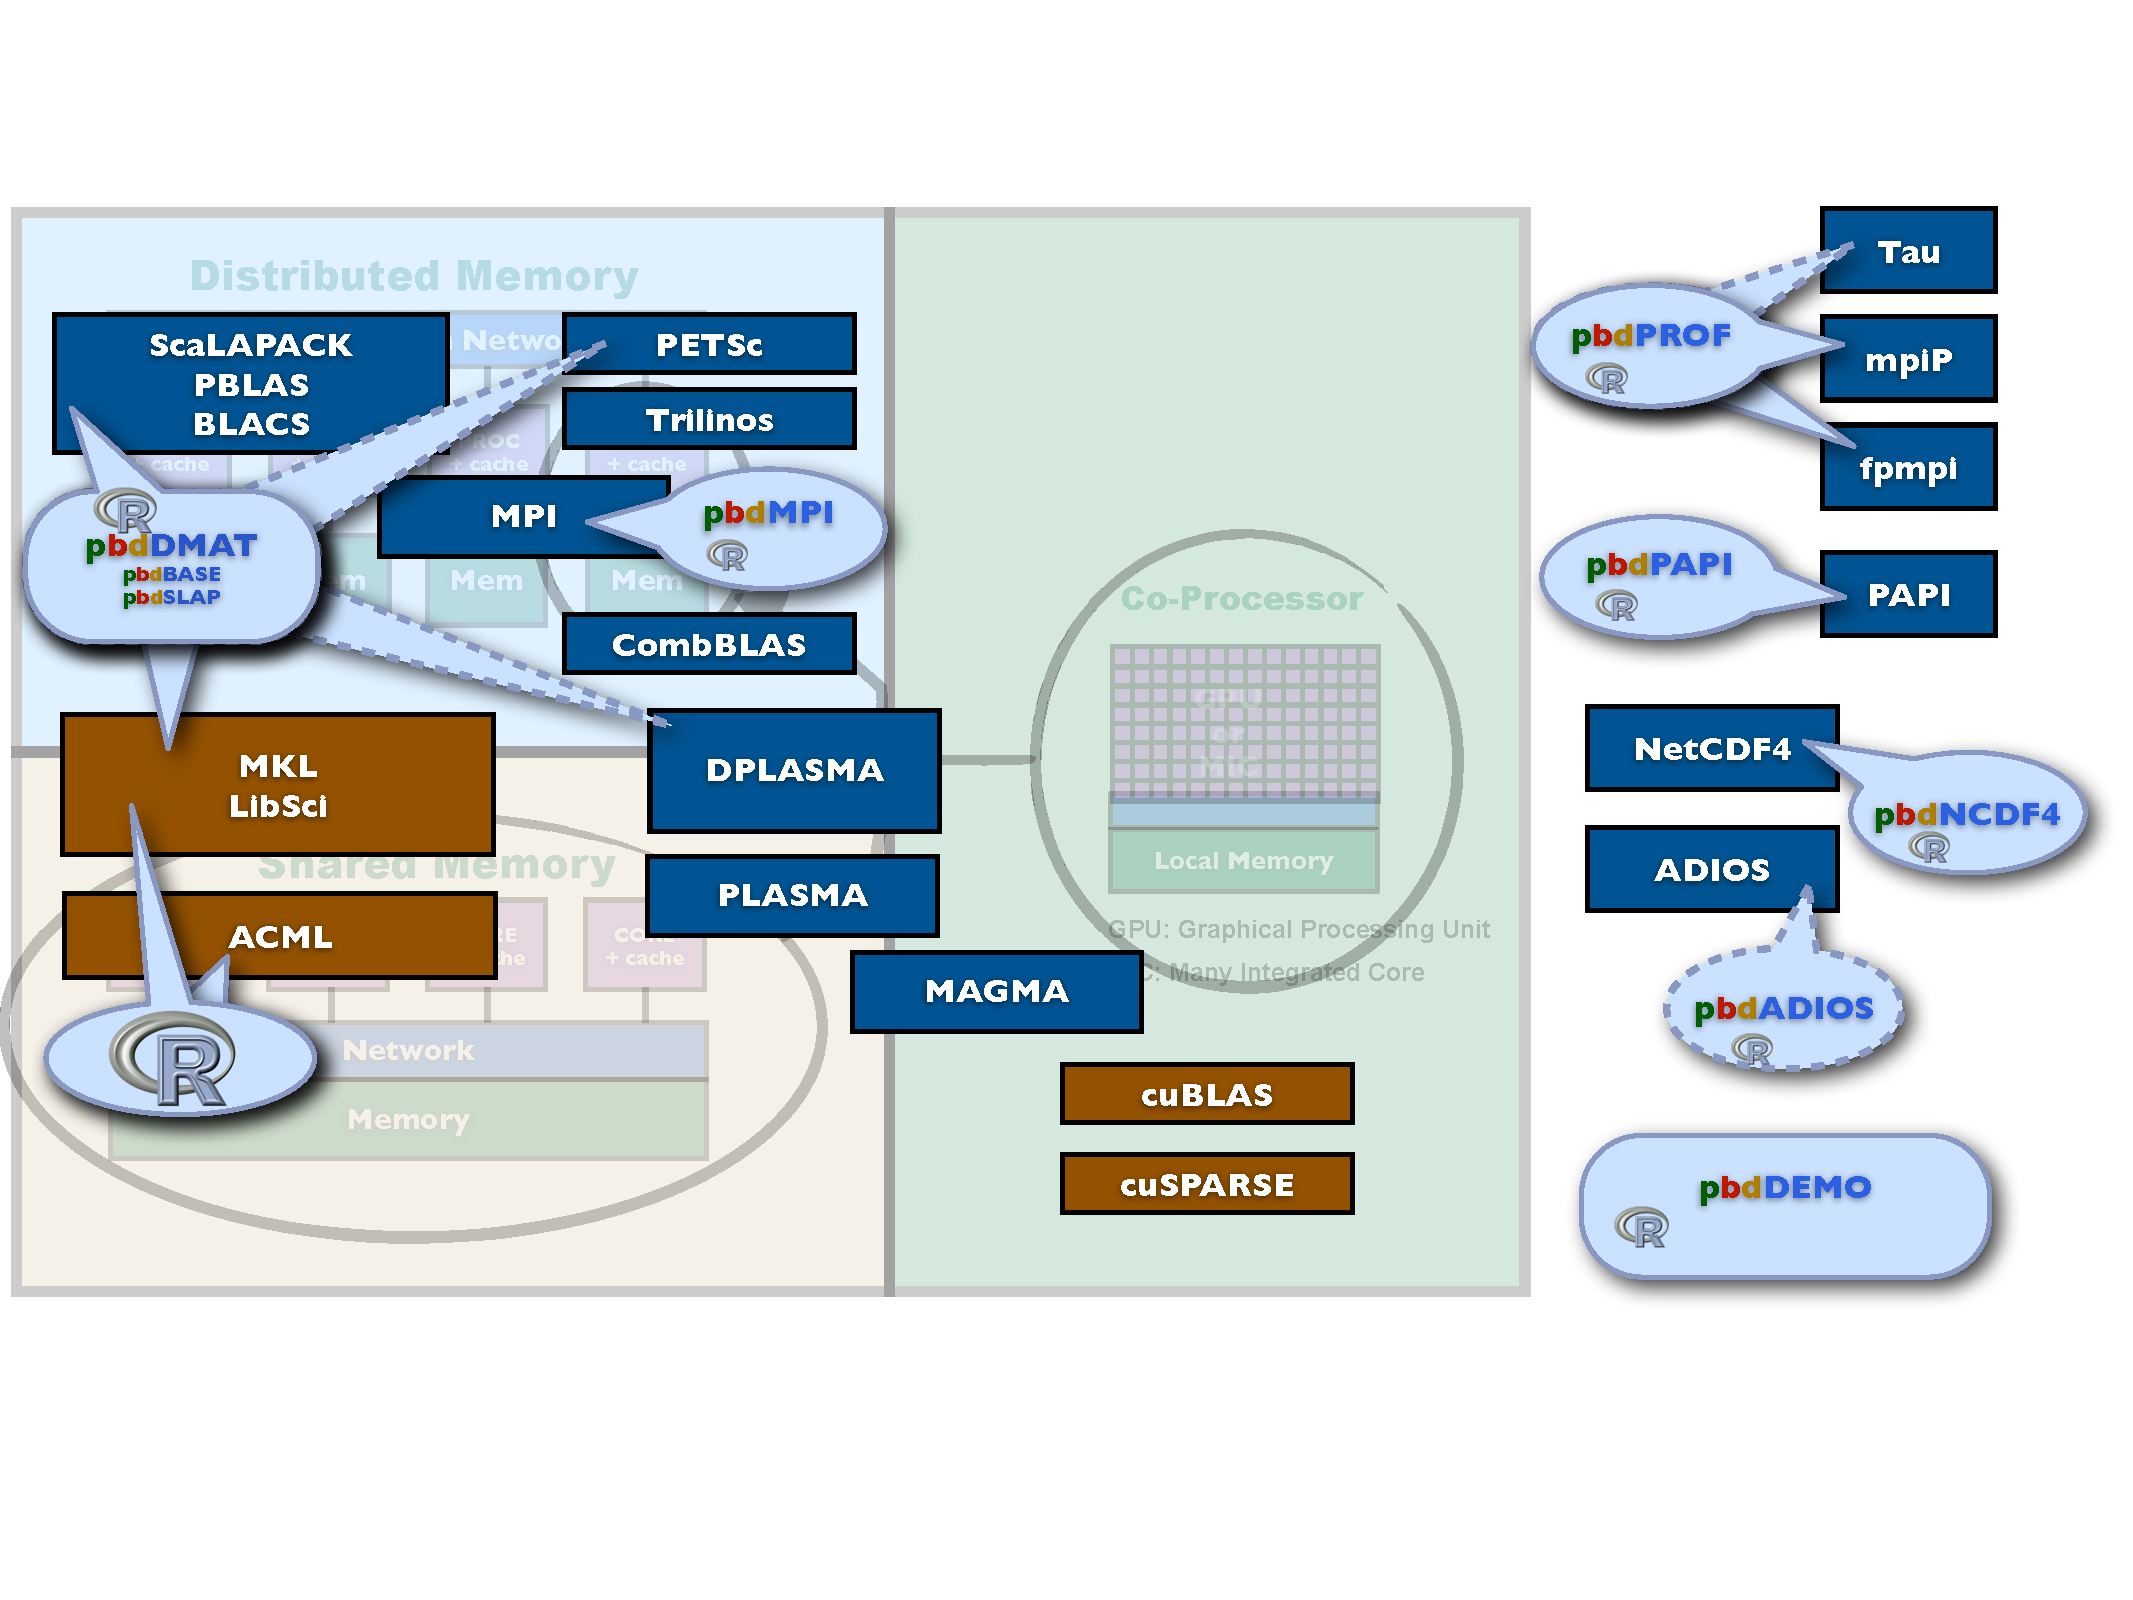
\includegraphics[trim=0cm 5cm 0cm 3cm,clip=true,width=0.85\textwidth]
  {../common/pics/hardware/ParallelHardware27.pdf}
  \scriptsize
  \begin{block}{Why use HPC libraries?}
    \begin{itemize}[<+-|alert@+>]
    \item The HPC community is 30 years beyond ``embarrassingly parallel.''
    \item \emph{They're tested.} \emph{They're
        fast.}  \emph{They're scalable.}
    \item Many science communities are invested in their API.
    \item Data analysis uses much of the same math as simulation science.
    \end{itemize}
  \end{block}
\end{frame}

\subsection{pbdMPI}
\makesubcontentsslidessec

\begin{frame}
  \begin{block}{pbdMPI: a High Level Interface to MPI}
    \begin{itemize}
    \item API is simplified: defaults in control objects.
    \item S4 methods: extensible to complex \R objects.
    \item Additional error checking
    \item Array and matrix methods without serialization: faster than
      \pkg{Rmpi}.
    \end{itemize}
    \begin{center}
      \vspace{0.2cm}\scriptsize
      \begin{tabular}{ll} \hline\hline
        \pkg{pbdMPI} (S4) & \pkg{Rmpi}                \\ \hline
        \code{\color{blue}allreduce}    & \code{mpi.allreduce}      \\
        \code{\color{blue}allgather}    & \code{mpi.allgather},
        \code{mpi.allgatherv},
        \code{mpi.allgather.Robj} \\
        \code{bcast}        & \code{mpi.bcast},
        \code{mpi.bcast.Robj}     \\
        \code{gather}       & \code{mpi.gather},
        \code{mpi.gatherv},
        \code{mpi.gather.Robj}    \\
        \code{recv}         & \code{mpi.recv},
        \code{mpi.recv.Robj}      \\
        \code{reduce}       & \code{mpi.reduce}         \\
        \code{scatter}      & \code{mpi.scatter},
        \code{mpi.scatterv},
        \code{mpi.scatter.Robj}   \\
        \code{send}         & \code{mpi.send},
        \code{mpi.send.Robj}      \\ \hline \hline
      \end{tabular}
    \end{center}
  \end{block}
\end{frame}

\begin{frame}[fragile]
  \begin{block}{Integer?\qquad Not always obvious in R.}
    \vspace{-.2cm}
    \begin{lstlisting}
> is.integer(1)
[1] FALSE
> is.integer(2)
[1] FALSE
> is.integer(1:2)
[1] TRUE
    \end{lstlisting}
  \end{block}
  \begin{block}{Often it's best to let the machine figure it out}\pause
    \begin{minipage}[t]{.475\textwidth}
      \begin{lstlisting}[title=Rmpi]
# int
mpi.allreduce(x, type=1)
# double
mpi.allreduce(x, type=2)
      \end{lstlisting}
    \end{minipage}
    \hfill
    \begin{minipage}[t]{.475\textwidth}
      \begin{lstlisting}[title=pbdMPI]
allreduce(x)
      \end{lstlisting}
      % \vspace{1em}
      % \hspace{1em}{\small S4. Batch only! (No spawning)}
    \end{minipage}
  \end{block}
\end{frame}



% \begin{frame}[fragile,shrink]
%   \begin{block}{Embarrassingly Parallel Computation}\pause
%     \vspace{-1ex}
%     \begin{minipage}[t]{.45\textwidth}
%       \begin{lstlisting}[title=EPforeach.R "asking for parallel",basicstyle=\tiny]
% library(doMPI, quiet=TRUE)
% cl <- startMPIcluster()
% registerDoMPI(cl)

% n <- 10
% myIn <- vector("list", n)

% myFun <- function(x) {
%   s <- sum(rnorm(10000))
%   rank <- mpi.comm.rank(comm=0)
%   return(paste(s, "from", rank))
% }

% results <- foreach(i = 1:n) %dopar% {
%   out <- myFun(myIn[[i]])
% }

% print(results)

% closeCluster(cl)
% mpi.quit()
%       \end{lstlisting}
%     \end{minipage}
%     \hfill
%     \begin{minipage}[t]{.5\textwidth}
%       \begin{lstlisting}[title=EPpbdR.R "thinking parallel",basicstyle=\tiny]
% library(pbdMPI, quiet=TRUE)
% init()

% myChunk <- get.jid(n <- 10)
% myIn <- vector("list", length(myChunk))
% myOut <- vector("list", length(myChunk))

% myFun = function(x) {
%   s <- sum(rnorm(10000))
%   rank <- comm.rank()
%   return(paste(s, "from", rank))
% }

% for(i in 1:length(myChunk)) {
%   myOut[[i]] <- myFun(myIn[[i]])
% }
% results <- gather(myOut)

% comm.print(results)
% finalize()
%       \end{lstlisting}
%     \end{minipage}
%   \end{block}
% \end{frame}


\begin{frame}[fragile]{SPMD Runs Many Copies of One Code}
  \begin{exampleblock}{SPMD Hello World: a ``map-reduce'' to all}
    \vspace{-1.5ex}
    \centering
    \begin{lstlisting}[title=map-reduce.r]
library(pbdMPI, quiet = TRUE)
init()

## Your "Map" code
n <- comm.rank() + 1

## Now "Reduce" but give the result to all
all_sum <- allreduce(n) # Sum is default

text <- paste("Hello: n is", n, "sum is", all_sum )
comm.print(text, all.rank=TRUE)

finalize()
    \end{lstlisting}
    \vspace{-4.5ex}
    \begin{columns}[t,onlytextwidth]
      \begin{column}{0.54\textwidth}
        \begin{lstlisting}[backgroundcolor=\color{white},keywordstyle=\color{black},
title=Execute this batch script via:]
mpirun -np 2 Rscript map-reduce.r
        \end{lstlisting}
      \end{column}
      \hfill
      \begin{column}{0.46\textwidth}
        \begin{lstlisting}[title=Output:]
COMM.RANK = 0
[1] "Hello: n is 1 sum is 3"
COMM.RANK = 1
[1] "Hello: n is 2 sum is 3"
        \end{lstlisting}
      \end{column}
    \end{columns}
  \end{exampleblock}
\end{frame}

\subsection{pbdDMAT}
\makesubcontentsslidessec

\begin{frame}{Dense Matrix and Vector Operations}
  \begin{block}{A matrix is mapped to a processor grid shape}
    \begin{table}[ht]
      \centering
      % \begin{subfigure}[b]{0.23\textwidth}
      %   \centering
      %   $\left[\begin{tabular}{l}
      %       0 \\ 1 \\ 2 \\ 3 \\ 4 \\ 5
      %     \end{tabular}\right]^T$
      %   \caption{$1\times 6$}
      % \end{subfigure}
      \begin{subfigure}[b]{0.23\textwidth}
        \centering
        $\left[\begin{tabular}{llllll}
            0 & 1 & 2 & 3 & 4 & 5
          \end{tabular}\right]$
        \vspace{1.5cm}
        \caption{$1\times 6$}
      \end{subfigure}%\hspace{-1cm}
      \begin{subfigure}[b]{0.23\textwidth}
        \centering
        $\left[\begin{tabular}{lll}
            0 & 1 & 2\\
            3 & 4 & 5
          \end{tabular}\right]$
        \caption{$2\times 3$}
      \end{subfigure}%
      \begin{subfigure}[b]{0.23\textwidth}
        \centering
        $\left[\begin{tabular}{ll}
            0 & 1 \\
            2 & 3\\
            4 & 5
          \end{tabular}\right]$
        \caption{$3\times 2$}
      \end{subfigure}
      \begin{subfigure}[b]{0.23\textwidth}
        \centering
        $\left[\begin{tabular}{l}
            0 \\ 1 \\ 2 \\ 3 \\ 4 \\ 5
          \end{tabular}\right]$
        \caption{$6\times 1$}
      \end{subfigure}
      \caption{Processor Grid Shapes with 6 Processors}\label{fig:gridshapes}
    \end{table}
  \end{block}
\end{frame}

\begin{frame}[shrink]
\begin{exampleblock}{2$\times$3 block-cyclic grid on 6 processors:
    Global view ``ddmatrix'' class}
\begin{align*}
x &= \left[
      \begin{array}{ll|ll|ll|ll|l}
      \color{g11}x_{11} & \color{g11}x_{12} & \color{g12}x_{13} & \color{g12}x_{14} & \color{g13}x_{15} & \color{g13}x_{16} & \color{g11}x_{17} & \color{g11}x_{18} & \color{g12}x_{19}\\
      \color{g11}x_{21} & \color{g11}x_{22} & \color{g12}x_{23} & \color{g12}x_{24} & \color{g13}x_{25} & \color{g13}x_{26} & \color{g11}x_{27} & \color{g11}x_{28} & \color{g12}x_{29}\\\hline
      \color{g21}x_{31} & \color{g21}x_{32} & \color{g22}x_{33} & \color{g22}x_{34} & \color{g23}x_{35} & \color{g23}x_{36} & \color{g21}x_{37} & \color{g21}x_{38} & \color{g22}x_{39}\\
      \color{g21}x_{41} & \color{g21}x_{42} & \color{g22}x_{43} & \color{g22}x_{44} & \color{g23}x_{45} & \color{g23}x_{46} & \color{g21}x_{47} & \color{g21}x_{48} & \color{g22}x_{49}\\\hline
      \color{g11}x_{51} & \color{g11}x_{52} & \color{g12}x_{53} & \color{g12}x_{54} & \color{g13}x_{55} & \color{g13}x_{56} & \color{g11}x_{57} & \color{g11}x_{58} & \color{g12}x_{59}\\
      \color{g11}x_{61} & \color{g11}x_{62} & \color{g12}x_{63} & \color{g12}x_{64} & \color{g13}x_{65} & \color{g13}x_{66} & \color{g11}x_{67} & \color{g11}x_{68} & \color{g12}x_{69}\\\hline
      \color{g21}x_{71} & \color{g21}x_{72} & \color{g22}x_{73} & \color{g22}x_{74} & \color{g23}x_{75} & \color{g23}x_{76} & \color{g21}x_{77} & \color{g21}x_{78} & \color{g22}x_{79}\\
      \color{g21}x_{81} & \color{g21}x_{82} & \color{g22}x_{83} & \color{g22}x_{84} & \color{g23}x_{85} & \color{g23}x_{86} & \color{g21}x_{87} & \color{g21}x_{88} & \color{g22}x_{89}\\\hline
      \color{g11}x_{91} & \color{g11}x_{92} & \color{g12}x_{93} & \color{g12}x_{94} & \color{g13}x_{95} & \color{g13}x_{96} & \color{g11}x_{97} & \color{g11}x_{98} & \color{g12}x_{99}\\
      \end{array}
\right]_{9\times 9}
\end{align*}
\begin{align*}
\text{Processor grid = }\left|
      \begin{array}{lll}
      \color{g11}0 & \color{g12}1 & \color{g13}2\\
      \color{g21}3 & \color{g22}4 & \color{g23}5
      \end{array}
\right| &=
\left|
      \begin{tabular}{lll}
      \color{g11}(0,0) & \color{g12}(0,1) & \color{g13}(0,2)\\
      \color{g21}(1,0) & \color{g22}(1,1) & \color{g23}(1,2)
      \end{tabular}
\right|
\end{align*}
\end{exampleblock}
\end{frame}


\begin{frame}[shrink]
\begin{exampleblock}{2$\times$3 block-cyclic grid on 6 processors:
    Local view ``ddmatrix'' class}
\begin{align*}
\left[
      \begin{array}{ll|ll}
      \color{g11}x_{11} & \color{g11}x_{12} & \color{g11}x_{17} & \color{g11}x_{18}\\
      \color{g11}x_{21} & \color{g11}x_{22} & \color{g11}x_{27} & \color{g11}x_{28}\\\hline
      \color{g11}x_{51} & \color{g11}x_{52} & \color{g11}x_{57} & \color{g11}x_{58}\\
      \color{g11}x_{61} & \color{g11}x_{62} & \color{g11}x_{67} & \color{g11}x_{68}\\\hline
      \color{g11}x_{91} & \color{g11}x_{92} & \color{g11}x_{97} & \color{g11}x_{98}\\
      \end{array}
\right]_{5\times 4}
\left[
      \begin{array}{ll|l}
      \color{g12}x_{13} & \color{g12}x_{14} & \color{g12}x_{19}\\
      \color{g12}x_{23} & \color{g12}x_{24} & \color{g12}x_{29}\\\hline
      \color{g12}x_{53} & \color{g12}x_{54} & \color{g12}x_{59}\\
      \color{g12}x_{63} & \color{g12}x_{64} & \color{g12}x_{69}\\\hline
      \color{g12}x_{93} & \color{g12}x_{94} & \color{g12}x_{99}\\
      \end{array}
\right]_{5\times 3}
\left[
      \begin{array}{ll}
      \color{g13}x_{15} & \color{g13}x_{16}\\
      \color{g13}x_{25} & \color{g13}x_{26}\\\hline
      \color{g13}x_{55} & \color{g13}x_{56}\\
      \color{g13}x_{65} & \color{g13}x_{66}\\\hline
      \color{g13}x_{95} & \color{g13}x_{96}\\
      \end{array}
\right]_{5\times 2}
\\
\left[
      \begin{array}{ll|ll}
      \color{g21}x_{31} & \color{g21}x_{32} & \color{g21}x_{37} & \color{g21}x_{38}\\
      \color{g21}x_{41} & \color{g21}x_{42} & \color{g21}x_{47} & \color{g21}x_{48}\\\hline
      \color{g21}x_{71} & \color{g21}x_{72} & \color{g21}x_{77} & \color{g21}x_{78}\\
      \color{g21}x_{81} & \color{g21}x_{82} & \color{g21}x_{87} & \color{g21}x_{88}\\
      \end{array}
\right]_{4\times 4}
\left[
      \begin{array}{ll|l}
      \color{g22}x_{33} & \color{g22}x_{34} & \color{g22}x_{39}\\
      \color{g22}x_{43} & \color{g22}x_{44} & \color{g22}x_{49}\\\hline
      \color{g22}x_{73} & \color{g22}x_{74} & \color{g22}x_{79}\\
      \color{g22}x_{83} & \color{g22}x_{84} & \color{g22}x_{89}\\
      \end{array}
\right]_{4\times 3}
\left[
      \begin{array}{ll}
      \color{g23}x_{35} & \color{g23}x_{36} \\
      \color{g23}x_{45} & \color{g23}x_{46} \\\hline
      \color{g23}x_{75} & \color{g23}x_{76} \\
      \color{g23}x_{85} & \color{g23}x_{86} \\
      \end{array}
\right]_{4\times 2}
\end{align*}
\begin{align*}
\text{Processor grid = }\left|
      \begin{array}{lll}
      \color{g11}0 & \color{g12}1 & \color{g13}2\\
      \color{g21}3 & \color{g22}4 & \color{g23}5
      \end{array}
\right| &=
\left|
      \begin{tabular}{lll}
      \color{g11}(0,0) & \color{g12}(0,1) & \color{g13}(0,2)\\
      \color{g21}(1,0) & \color{g22}(1,1) & \color{g23}(1,2)
      \end{tabular}
\right|
\end{align*}
\end{exampleblock}
\end{frame}

\begin{frame}[fragile]
  \begin{block}{\pbdR\ No change in syntax. \hfill Data redistribution functions.}
\vspace{-2ex}
  \begin{lstlisting}
x <- x[-1, 2:5]
x <- log(abs(x) + 1)
x.pca <- prcomp(x)
xtx <- t(x) %*% x
ans <- svd(solve(xtx))
  \end{lstlisting}
\vspace{-1ex}
  \begin{center}
  \emph{The above (and over 100 other functions) runs on 1 core with R \\
    or 10,000 cores with \pbdR ddmatrix class}
  \end{center}
\vspace{-2ex}
\begin{lstlisting}
> showClass("ddmatrix")
Class "ddmatrix" [package "pbdDMAT"]
Slots:
Name:     Data     dim    ldim   bldim   ICTXT
Class:  matrix numeric numeric numeric numeric
\end{lstlisting}
\vspace{-2ex}
\begin{lstlisting}
> x <- as.rowblock(x)
> x <- as.colblock(x)
> x <- redistribute(x, bldim=c(8, 8), ICTXT = 0)
\end{lstlisting}
  \end{block}
\end{frame}

\input{../common/06_dmatstats/randsvd.tex}



\section{Benchmarks}

\hidenum
\begin{frame}[noframenumbering]
\frametitle{Contents}
 \tableofcontents[currentsection,hideallsubsections]
\end{frame}
\shownum

\subsection{Productivity Benchmark}

\begin{frame}[fragile]
\fontsize{8pt}{10}\selectfont
\begin{block}{Truncated SVD from Random Projections\footnotemark}
  \begin{minipage}{.55\textwidth}
    \begin{center}
      \includegraphics[width=.95\textwidth]{../common/pics/randSVDalg}
      \\
      \includegraphics[width=.95\textwidth]{../common/pics/randSVDalg4_4}
    \end{center}
  \end{minipage}
%   \hspace{.01cm}
  \begin{minipage}{0.430\textwidth}
\begin{lstlisting}[title=Serial 
R,basicstyle=\tiny,backgroundcolor=\color{grayish} 
,numberstyle=\tiny\color{black},keywordstyle=\color{black},commentstyle=\color{ 
dkgreen},stringstyle=\color{black},escapeinside={(*@}{@*)}]
randSVD <- function(A, k, q=3)
  {
    ## Stage A
    Omega <- (*@ matrix(rnorm(n*2*k),@*) 
            (*@ nrow=n, ncol=2*k) @*)
    Y <- A %*% Omega
    Q <- qr.Q(qr(Y))
    At <- t(A)
    for(i in 1:q)
      {
        Y <- At %*% Q
        Q <- qr.Q(qr(Y))
        Y <- A %*% Q
        Q <- qr.Q(qr(Y))
      }
    
    ## Stage B
    B <- t(Q) %*% A
    U <- La.svd(B)$u
    U <- Q %*% U
    U[, 1:k]
  }
\end{lstlisting} %balance$
\end{minipage}
{\fontsize{6pt}{10}\selectfont $^1$Halko, Martinsson, 
  and Tropp, 2011. Finding structure with randomness: probabilistic algorithms 
  for constructing approximate matrix decompositions \emph{SIAM Review} \textbf{53} 
  217--288}
\end{block}
\end{frame}


\begin{frame}[fragile]
 \fontsize{8pt}{10}\selectfont
\begin{block}{Randomized SVD}
  \hfill
  \begin{minipage}{0.430\textwidth}
\begin{lstlisting}[title=Serial 
R,basicstyle=\tiny,backgroundcolor=\color{grayish} 
,numberstyle=\tiny\color{black},keywordstyle=\color{black},commentstyle=\color{ 
dkgreen},stringstyle=\color{black},escapeinside={(*@}{@*)}]
randSVD <- function(A, k, q=3)
  {
    ## Stage A
    Omega <- (*@ \textcolor{blue}{matrix(rnorm(n*2*k),} @*) 
         (*@ \textcolor{blue}{ nrow=n, ncol=2*k)} @*)
    Y <- A %*% Omega
    Q <- qr.Q(qr(Y))
    At <- t(A)
    for(i in 1:q)
      {
        Y <- At %*% Q
        Q <- qr.Q(qr(Y))
        Y <- A %*% Q
        Q <- qr.Q(qr(Y))
      }
    
    ## Stage B
    B <- t(Q) %*% A
    U <- La.svd(B)$u
    U <- Q %*% U
    U[, 1:k]
  }
\end{lstlisting} %balance$
  \end{minipage}
  \hfill
  \begin{minipage}{0.430\textwidth}
\begin{lstlisting}[title=Parallel pbdR,basicstyle=\tiny,backgroundcolor=\color{
grayish}, numberstyle=\tiny\color{black},keywordstyle=\color{black},
commentstyle=\color{dkgreen},stringstyle=\color{black},escapeinside={(*@}{@*)}]
randSVD <- function(A, k, q=3)
  {
    ## Stage A
    Omega <- (*@ \textcolor{blue}{ddmatrix("rnorm",} @*)
         (*@ \textcolor{blue}{nrow=n, ncol=2*k)} @*)
    Y <- A %*% Omega
    Q <- qr.Q(qr(Y))
    At <- t(A)      
    for(i in 1:q)
      {
        Y <- At %*% Q   
        Q <- qr.Q(qr(Y))
        Y <- A %*% Q    
        Q <- qr.Q(qr(Y))
      }
    
    ## Stage B
    B <- t(Q) %*% A     
    U <- La.svd(B)$u 
    U <- Q %*% U     
    U[, 1:k]
  }
\end{lstlisting}  % balancing $
  \end{minipage}
\hfill
\end{block}
\end{frame}

\begin{frame}
  \begin{block}{Randomized SVD}
    \begin{center}
      \includegraphics[width=.45\textwidth]{../common/pics/randSVDspeedup}
      \hfill
      \includegraphics[width=.45\textwidth]{../common/pics/randSpeedupSVD}
    \end{center}
  \end{block}
\end{frame}

\subsection{Scalability Benchmarks}

\begin{frame}
  \begin{block}{Non-Optimal Choices Throughout}
    \begin{enumerate}[<+-|alert@+>]
      \item Only libre software used (no MKL, ACML, etc.).
      \item 1 core = 1 MPI process.
      \item No tuning for data layout.
    \end{enumerate}
  \end{block}
  \begin{block}{Benchmark Data}
    \begin{enumerate}[<+-|alert@+>]
      \item Random normal $N(100, 10000)$.
      \item Local problem size of $\approx 45.5 MB$.
      \item Three sets:  500, 1000, and 2000 columns.
      \item Several runs at different core sizes within each set.
    \end{enumerate}
  \end{block}
\end{frame}



% \subsection{Covariance}

\begin{frame}[fragile]
  \begin{block}{Covariance Code}
\begin{lstlisting}
x <- ddmatrix("rnorm", nrow=n, ncol=p, mean=mean, sd=sd)

cov.x <- cov(x)
\end{lstlisting}
  \end{block}
\end{frame}

\begin{frame}
  \begin{block}{\code{cov()}}
  \begin{center}
    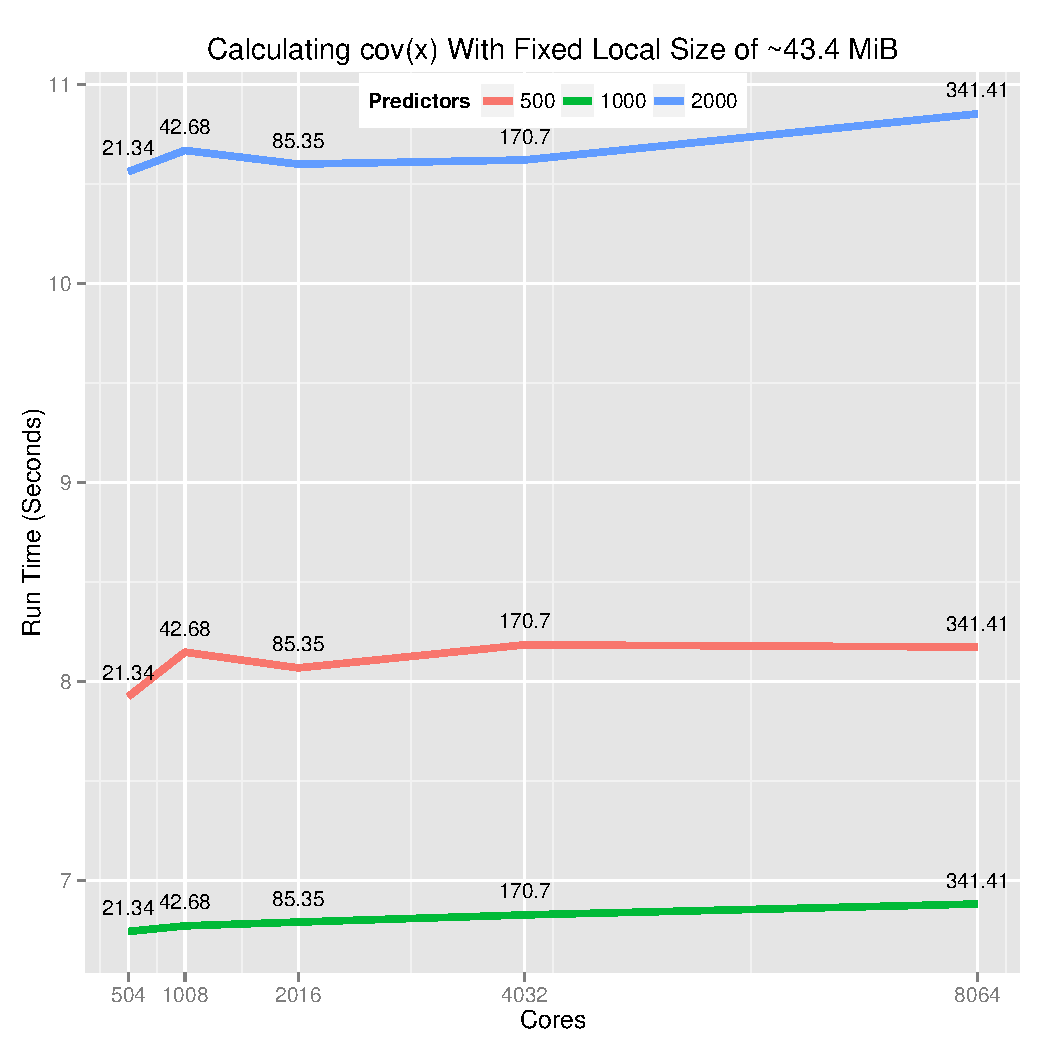
\includegraphics[height=.88\textheight]{../common/pics/cov}
  \end{center}
  \end{block}
\end{frame}



% \subsection{Linear Model Fitting}

\begin{frame}[fragile]
  \begin{block}{Linear Model Code}
\begin{lstlisting}
x <- ddmatrix("rnorm", nrow=n, ncol=p, mean=mean, sd=sd)
beta_true <- ddmatrix("runif", nrow=p, ncol=1)

y <- x %*% beta_true

beta_est <- lm.fit(x=x, y=y)$coefficients 
\end{lstlisting}
  \end{block}
\end{frame}

\begin{frame}
  \begin{block}{\code{Data Generation}}
  \begin{center}
    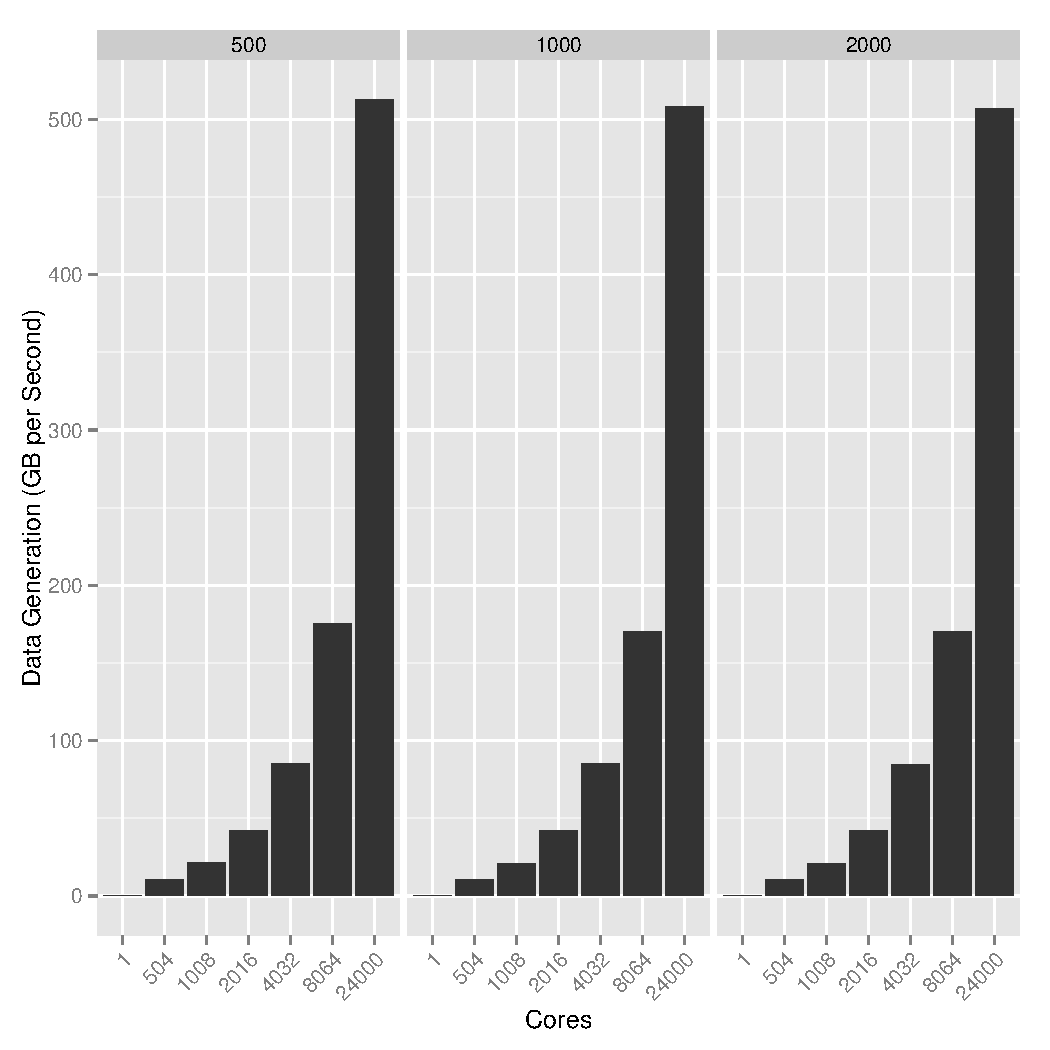
\includegraphics[height=.88\textheight]{../common/pics/datagen}
  \end{center}
  \end{block}
\end{frame}

% \begin{frame}
%   \begin{block}{\code{lm.fit()}}
%   \begin{center}
%     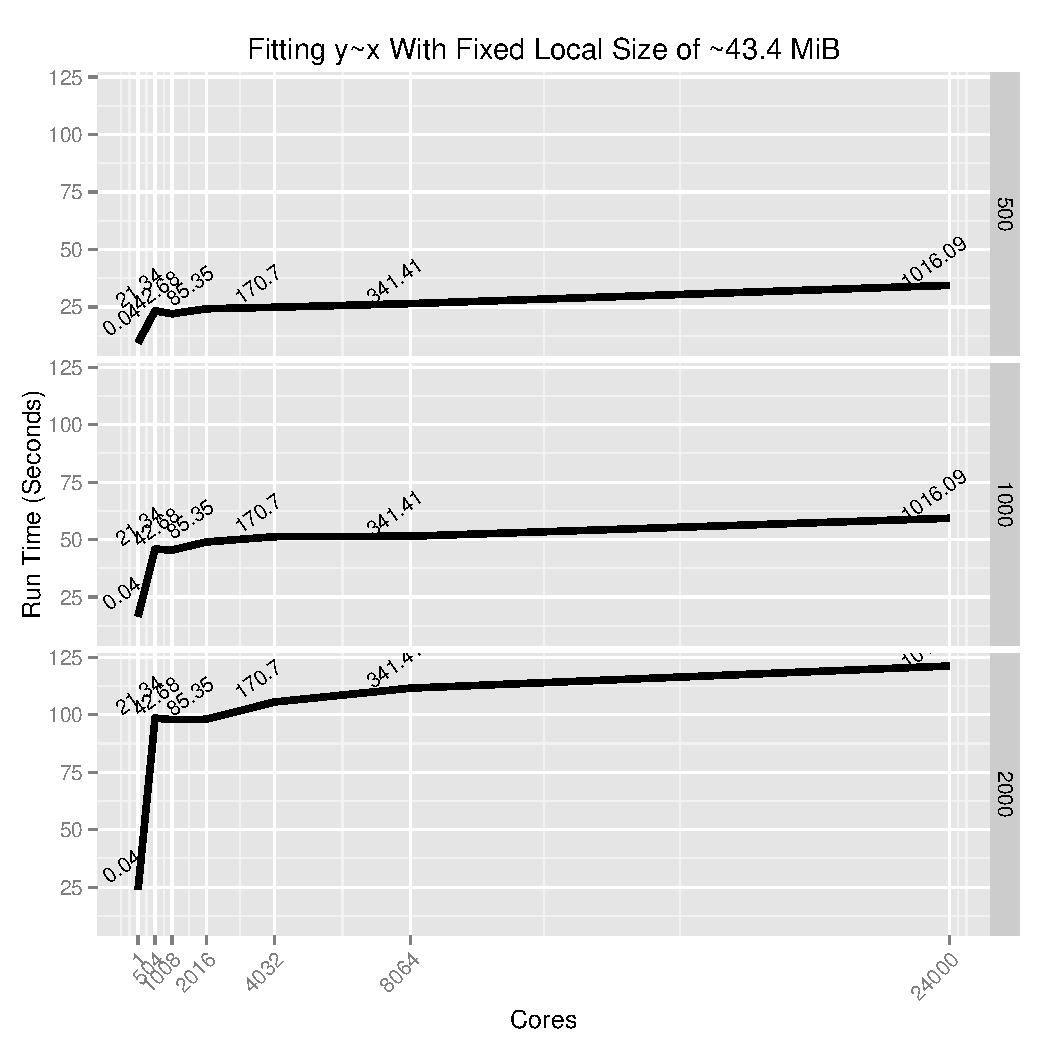
\includegraphics[height=.88\textheight]{../common/pics/lmfit1}
%   \end{center}
%   \end{block}
% \end{frame}

\begin{frame}
  \begin{block}{\code{lm.fit()}}
  \begin{center}
    \includegraphics[height=.88\textheight]{../common/pics/lmfit2}
  \end{center}
  \end{block}
\end{frame}
\section{Challenges}

\hidenum
\begin{frame}[noframenumbering]
\frametitle{Contents}
 \tableofcontents[currentsection,hideallsubsections]
\end{frame}
\shownum


\subsection{Challenges}

\begin{frame}
  \begin{block}{Challenges}
    \begin{itemize}[<+-|alert@+>]
      \item Perceptions.
      \item Library loading.
      \item Profiling.
    \end{itemize}
  \end{block}
\end{frame}


\begin{frame}
  \begin{block}{Covariance Revisited: Distributed Data Parameter Calibration}
    \begin{center}
     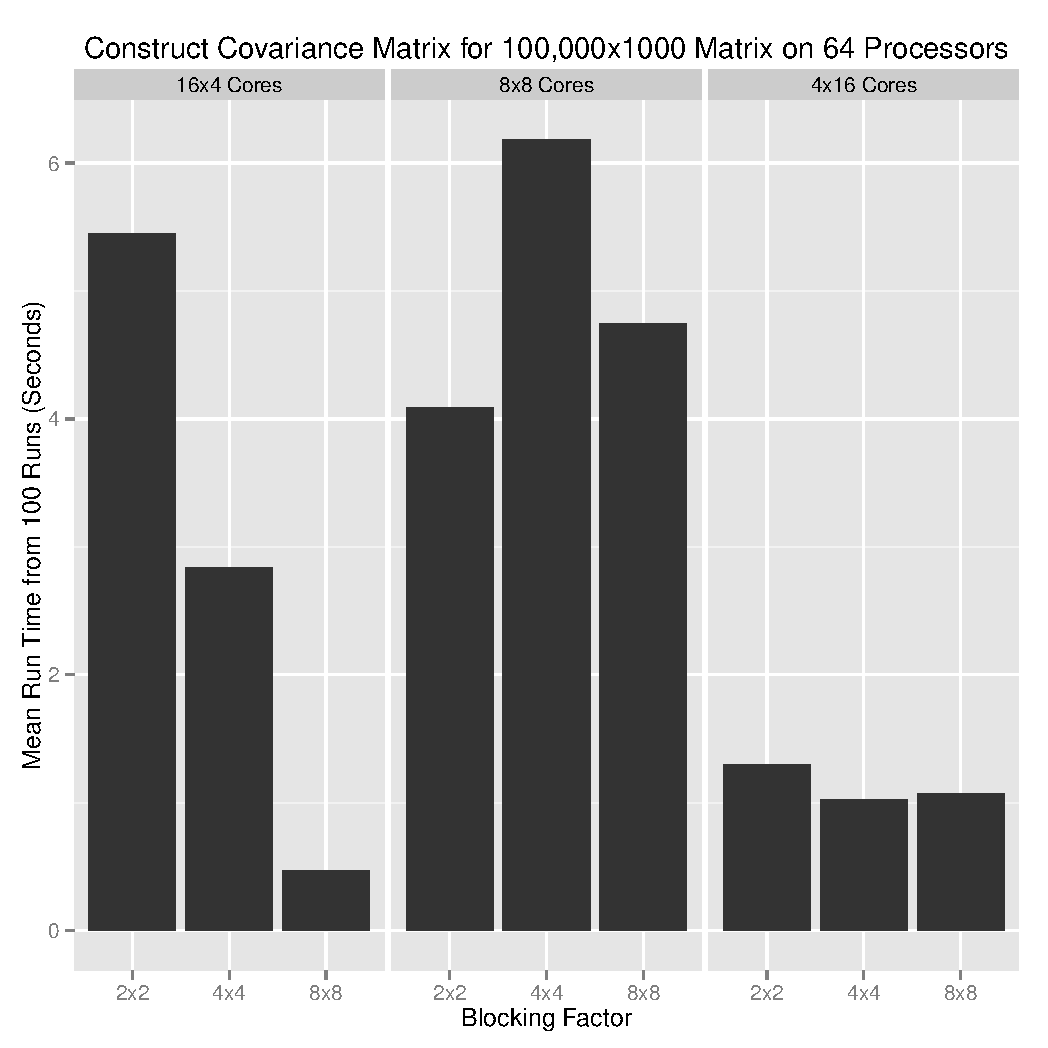
\includegraphics[width=10cm, height=7cm]{../common/pics/cov_param}
    \end{center}
  \end{block}
\end{frame}

\begin{frame}
  \begin{block}{Adding More Levels of Parallelism}
    \begin{center}
      {\color{dkblue}Distributed Memory (cluster nodes)} \\
      {\color{dkgreen}Shared Memory (multicore)} \\
      {\color{purple}Co-Processor (GPU, manycore)}
    \end{center}
    \begin{itemize}
      \item {\color{dkblue}pbdDMAT} + {\color{purple}CUBLAS}: near term on Titan 
      \item {\color{dkblue}pbdDMAT} - {\color{dkblue}ScaLAPACK} +
        {\color{dkblue}D}{\color{dkgreen}PLASMA}: QR only 
      \item {\color{dkblue}pbdDMAT} + {\color{dkgreen}PLASMA} or
        {\color{dkgreen}MKL} or {\color{dkgreen}ACML}: often helps 
      \item {\color{dkblue}pbdDMAT} + {\color{purple}MAGMA}: may not help 
    \end{itemize}
  \end{block}
\end{frame}

\hidenum
\section*{}
\begin{frame}[noframenumbering]
  \begin{block}{Tutorials}
  \begin{itemize}
    \item {\small OLCF Very Large Data Workshop
         ... {\color{red} NEXT!}}
    \item {\small Seoul National University, August 20}
    \item {\small SC13, November 17-22, Denver}
  \end{itemize}
  \end{block}
  \begin{block}{Invited Talks}
  \begin{itemize}
    \item {\small International Association for Statistical Computing, Aug 22-23, Seoul}
    \item {\small 59th ISI World Statistics Congress, August 25-30, Hong Kong }
  \end{itemize}
  \end{block}
\end{frame}
  
\begin{frame}[noframenumbering]
 \begin{block}{Thanks for coming!}
 \begin{center}
     {\Large Questions?}\\[1cm]
     {\Large Be sure to stick around for the tutorial!}
  \end{center}
 \end{block}
\end{frame}


\end{document}
% -------------------------------------------------------------------------
% Logos
% -------------------------------------------------------------------------

\definecolor{ORNL}{HTML}{008752}
\definecolor{UT}{HTML}{F77F00}
\setbeamercolor{title}{fg=white}
\setbeamercolor{frametitle}{fg=white}


\newcommand{\titlelogos}{}

\newcommand{\utpres}{
\renewcommand*\titlelogos{\centering
\includegraphics[scale=.6]{%
../common/pics/logos/logos_ut}}
  \logo{
\includegraphics[height=.34cm]{../common/pics/logos/utk.png}}
  \setbeamercolor{structure}{fg=UT}
}

\newcommand{\ornlpres}{
\renewcommand*\titlelogos{\centering
\includegraphics[scale=.6]{%
../common/pics/logos/logos_ornl}}
  \logo{
\includegraphics[height=.34cm]{../common/pics/logos/ornl.jpg}}
  \setbeamercolor{structure}{fg=ORNL}
}

\newcommand{\allpres}{
  \renewcommand*\titlelogos{\centering%
  
\includegraphics[scale=.6]{../common/pics/logos/logos_all}}

  \logo{\begin{tabular}{r}\includegraphics[height=.34cm]%
  {../common/pics/logos/utk.png} \\ 
  \includegraphics[height=.34cm]%
  {../common/pics/logos/ornl.jpg}\end{tabular}}
  \setbeamercolor{structure}{fg=UT}
}

\newcommand{\allpresou}{
\renewcommand*\titlelogos{\centering
\includegraphics[scale=.6]{%
../common/pics/logos/logos_all}}
  \logo{\begin{tabular}{r}
\includegraphics[height=.34cm]{%
          ../common/pics/logos/ornl.jpg} \\ 

\includegraphics[height=.34cm]{../common/pics/logos/utk.png}\end{tabular}}
  \setbeamercolor{structure}{fg=ORNL}
}



% -------------------------------------------------------------------------
% Subsection contents slides
% -------------------------------------------------------------------------

\newcommand{\makesubcontentsslides}{
  \hidenum
\begin{frame}[noframenumbering]
\frametitle{Contents}
 \tableofcontents[currentsection,hideothersubsections,sectionstyle=show/hide]
\end{frame}
\shownum
}

\newcommand{\makesubcontentsslidessec}{
  \hidenum
\begin{frame}[noframenumbering]
\tableofcontents[currentsection,
  sectionstyle=show/show,
  subsectionstyle=show/shaded/hide]
\end{frame}
\shownum
}


\usepackage{xcolor}

\definecolor{gray}{rgb}{.6,.6,.6}
\definecolor{orange}{rgb}{1,0.5,0}
\definecolor{grayish}{rgb}{.875, .875, .875}
\definecolor{dkgray}{rgb}{.375, .375, .375}
\definecolor{dkgreen}{rgb}{0,0.6,0}
\definecolor{mauve}{rgb}{0.58,0,0.82}
\definecolor{dkblue}{rgb}{0, 0, .5}

\definecolor{g11}{rgb}{0, 0, 1}
\definecolor{g12}{rgb}{0, .4, 1}
\definecolor{g13}{rgb}{0, .8, 1}

\definecolor{g21}{rgb}{0, .5, .3}
\definecolor{g22}{rgb}{.4, .5, .3}
\definecolor{g23}{rgb}{.8, .5, .3}
\usepackage{listings}

\lstset{ %
  language=R,     
  numbers=left,
  stepnumber=1,       
  numbersep=6pt,      
  showspaces=false,      
  showstringspaces=false,  
  showtabs=false,    
  frame=single,      
  rulecolor=\color{black},   
  tabsize=4,     
  captionpos=t,     
  breaklines=true,     
  breakatwhitespace=true,   
  title=\lstname,              
  basicstyle=\ttfamily\color{black}\scriptsize, 
  backgroundcolor=\color{grayish},  
  numberstyle=\tiny\color{black},  
  keywordstyle=\color{blue}, 
  commentstyle=\color{dkgreen}, 
  stringstyle=\color{mauve}, 
  xleftmargin=.1in,
  xrightmargin=.1in,
  aboveskip=0cm,
  belowskip=.2cm
  %   escapeinside={\%*}{*)},    
%   morekeywords={*,...}    
}


\lstdefinelanguage{shl}{
  language=sh,
  backgroundcolor=\color{white},
  basicstyle=\scriptsize\ttfamily\color{black},
  keywordstyle=\color{blue},
  commentstyle=\color{dkgreen},
  stringstyle=\color{mauve},
  numbers=none
}


\lstdefinelanguage{Rinteractive}{
  language=Sh,
  backgroundcolor=\color{white},
  basicstyle=\scriptsize\ttfamily\color{black},
  keywordstyle=\color{black},
  commentstyle=\color{black},
  stringstyle=\color{black},
  numbers=none
}


\lstdefinelanguage{Rcpp}{
        language=C++,
        basicstyle=\ttfamily\color{black}\scriptsize,
        backgroundcolor=\color{white},
        frame=single,
        breaklines=true,
        keywordstyle=\color{blue},
        commentstyle=\color{dkgreen}\itshape,
        stringstyle=\color{mauve},
        numbers=none,
        showspaces=false,
        showstringspaces=false,
        showtabs=false,
        rulecolor=\color{gray},
        tabsize=4,
        captionpos=t,
        morecomment=[l]{//},
        morekeywords={%
    % Rcpp
    Wrap, RcppExport, NumericVector, NumericMatrix, IntegerVector, 
IntegerMatrix, 
    Rcout, Rcpp, std, endl,
    % Native
    PROTECT, allocVector, allocMatrix, VECSXP, R_NilValue, SEXP,
    INTEGER, REAL
  }
}





\usepackage{tikz} 
\def\Put(#1,#2)#3{\leavevmode\makebox(0,0){\put(#1,#2){#3}}}


\usepackage{amsmath}
\usepackage{beamerthemesplit}
\usepackage{fancybox}
\usepackage{hyperref}
\usepackage[compatibility=false]{caption}
\usepackage{subcaption}


\makeatletter
\newcommand\code{\bgroup\@makeother\_\@makeother\~\@makeother\$\@codex}
\def\@codex#1{{\normalfont\ttfamily\hyphenchar\font=-1 #1}\egroup}
\makeatother

\newcommand{\bX}{\boldsymbol{X}}
\newcommand{\bx}{\boldsymbol{x}}
\newcommand{\by}{\boldsymbol{y}}
\newcommand{\bbeta}{\boldsymbol{\beta}}
\newcommand{\bepsilon}{\boldsymbol{\epsilon}}
\newcommand{\bs}[1]{\boldsymbol{#1}}



\setbeamertemplate{navigation symbols}{} 

\hypersetup{
    linkcolor=,
    colorlinks=true,
    urlcolor=blue
}

\usetheme{Frankfurt}
% \usecolortheme{whale}
% \usetheme{Antibes}
% \setbeamertemplate{mini frames}{}


\newcommand{\fctn}[1]{\textcolor{green!50!blue}{#1}}
\newcommand{\rfor}[1]{\textcolor{yellow!50!red}{#1}}
\newcommand{\rcom}[1]{\textcolor{blue}{#1}}

\newcommand{\pkg}[1]{\textbf{#1}}

\newcommand{\startr}{\begin{minipage}{.04\textwidth}\ \ \end{minipage} \begin{minipage}{.91\textwidth}}

%
\newcommand{\shownum}{\myfulltitle{\mytitlea}}
\newcommand{\hidenum}{\myfulltitle{\mytitleb}}
% \newcommand{\shownum}{\mytitle{\mytitlea}}
% \newcommand{\hidenum}{\mytitle{\mytitleb}}
% \expandafter\def\expandafter\insertshorttitle\expandafter{\insertshorttitle\hfill\insertframenumber\,/\,\inserttotalframenumber}
 

\newcounter{excount}
\setcounter{excount}{0}
\newcommand{\countex}{\addtocounter{excount}{1}\arabic{excount}}
\newcommand{\showex}{\arabic{excount}}





%%%%%%%%%%%%%%%%%%%%%%%%%%%%%%%%%%%%%%%%%%%%%%%%%%%%%%%%%%%%%%%%%%%%%%%%%%%%%%%
% \useoutertheme{miniframes}
\useoutertheme{infolines}

\makeatletter
\setbeamertemplate{footline}
{
  \leavevmode%
  \hbox{%
  \begin{beamercolorbox}[wd=.5\paperwidth,ht=2.25ex,dp=1ex,center]%
  {author in head/foot}%
    \usebeamerfont{author in head/foot}%
    \makebox[.48\paperwidth]%
      {\@myurl \hfill \@myshortauthor}
  \end{beamercolorbox}%
  \begin{beamercolorbox}[wd=.5\paperwidth,ht=2.25ex,dp=1ex,left]%
  {date in head/foot}%
   \hspace{1ex} \usebeamerfont{title in head/foot}\@myfulltitle
  \end{beamercolorbox}}%
  \vskip0pt%
}
\makeatother

\makeatletter
  \beamer@compressfalse
\makeatother




\setbeamertemplate{blocks}[rounded][shadow=false]
\addtobeamertemplate{block begin}{\pgfsetfillopacity{0.9}}{\pgfsetfillopacity{1}}
\setbeamercolor*{block title example}{fg=black,bg=blue!20}
\setbeamercolor*{block body example}{fg=black,bg=blue!5}



\allpresou
\neutralbg

\myfulltitle{Taking Statistical Computing to Parallel Platforms \\
  with R and pbdR}
\myabbrvtitle{Parallel Statistical Computing}
\myauthor{George Ostrouchov\\[1ex]
  Oak Ridge National Laboratory and University of Tennessee}
\myshortauthor{\pbdR Core Team}
\mydate{\textcolor{blue}{UTK Business Analytics and
    Statistics \\
Knoxville, February 27, 2015}} % insert conference title

%%%%%%%%%%%%%%%%%%%%%%%%%%%%%%%%%%%%%%%%%%%%%%%%%%%%%%%%%%%%%%%
\begin{document}

%%%%%%%%%%%%%%%%%%%%%%%%%%%%%%%%%%%%%%%%
%%     Title and ToC
%%%%%%%%%%%%%%%%%%%%%%%%%%%%%%%%%%%%%%%%
% titlepage
\frame{\maketitle}

\setcounter{footnote}{0}

\begin{frame}[noframenumbering]
\frametitle{The \pbdR\ Core Team}
\begin{minipage}{1\textwidth}
  \vspace{-.6cm}
\begin{minipage}{3.6cm}
\ \\[.8cm]
Wei-Chen Chen$^1$ \\
George Ostrouchov$^{2,3}$ \\
Pragneshkumar Patel$^3$ \\
Drew Schmidt$^3$\\[2ex]
\end{minipage}
\begin{minipage}{7cm}
  \ \hfill 
\includegraphics[width=5.5cm]{../common/pics/logos/newpbdr}
\end{minipage}
\end{minipage}
  \begin{minipage}{2.2cm}\tiny
    $^1$FDA\\
    Washington, DC, USA
  \end{minipage}
  \hspace{1ex}
  \begin{minipage}{5cm}\tiny
    $^2$Computer Science and Mathematics Division\\
    Oak Ridge National Laboratory, Oak Ridge TN, USA
  \end{minipage}
  \hspace{1ex}
  \begin{minipage}{4cm}\tiny
    $^3$Joint Institute for Computational Sciences\\
    University of Tennessee, Knoxville TN, USA
  \end{minipage}

\begin{block}{Support}\tiny
  This material is based upon work supported by the National Science
  Foundation Division of Mathematical Sciences under Grant No. 1418195.
  This work used resources of the \textcolor{blue}{National Institute for
  Computational Sciences} at the University of Tennessee, Knoxville,
  which is supported by the Office of Cyberinfrastructure of the
  U.S. National Science Foundation under Award  No. ARRA-NSF-OCI-0906324
  for NICS-RDAV center.
  This work also used resources of the \textcolor{blue}{Oak Ridge
  Leadership Computing Facility} at the Oak Ridge National
  Laboratory, which is supported by the Office of Science of the
  U.S. Department of Energy under Contract No. DE-AC05-00OR22725.\\[.2cm]
\end{block}
\end{frame}

\begin{frame}
  \frametitle{About This Presentation}
  \begin{block}{Downloads}\scriptsize
    You can update the \pbdR presentations and scripts in your virtual
    machine with: \\ \tt
    \$ cd \\
    \$ scp USERNAME@anselm.it4i.cz:/home/adios/slides/pbdr\_overview.pdf slides \\
    \$ scp
    USERNAME@anselm.it4i.cz:/home/adios/slides/pbdr\_tutorial.pdf
    slides \\
    rm -r scripts \\
    \$ scp -r USERNAME@anselm.it4i.cz:/home/adios/pbdR/scripts .
 \end{block}
\end{frame}

% \begin{frame}
% \frametitle{About This Presentation}
%   \begin{block}{Tutorial Evaluations}
%     \begin{center}
%       \url{http://bit.ly/sc13-tut-mf08}
%     \end{center}
%   \end{block}
% \end{frame}


\begin{frame}
\frametitle{About This Presentation}
 \begin{block}{Installation Instructions}
  Installation instructions for setting up a \pbdR environment are available:
  \begin{center}
  \url{http://r-pbd.org/install.html}
  \end{center}
  This includes instructions for installing R, MPI, and \pbdR.
 \end{block}
\end{frame}

% \begin{frame}%[allowframebreaks=0.8]
% \frametitle{About This Presentation}
%  \begin{block}{Conventions}
%   \begin{itemize}
%     \item We use ``{\Huge$ .$}'' as a decimal mark, not ``{\Huge$,$}''.  E.g.,
% 	``one thousand and one half'' is written ``$1,000.5$'', not ``$1.000,5$''.
%     \item We will use special suffixes to denote distributed objects (ones not
% 	stored entirely on a single processor).\\
%     \code{.spmd} denotes a distributed object, while\\
%     \code{.dmat} denotes a distributed object which is of class
% 	\code{ddmatrix}\\
%     No suffix means the object is global (common to all processors)\\[.2cm]
%     Neither of these suffices carries semantic meaning.
%     \end{itemize}
%  \end{block}
% \end{frame}



% \begin{frame}[fragile]
% \frametitle{About This Presentation}
%  \begin{block}{Conventions For Code Presentation}
% We will use two different forms of syntax highlighting.  One for displaying
% results from an interactive R session:
% \begin{lstlisting}[backgroundcolor=\color{white},basicstyle=\ttfamily\color{
% dkgray}\scriptsize,keywordstyle=\color{black},
%   commentstyle=\color{orange},stringstyle=\color{mauve}]
% R> "interactive"
% [1] "interactive"
% \end{lstlisting}
% and one for presenting R scripts
% \begin{lstlisting}
% "not interactive"
% \end{lstlisting}
%  \end{block}
% \end{frame}



\begin{frame}[noframenumbering,shrink]
\frametitle{Contents}
\small
\tableofcontents[hideallsubsections]
\end{frame}

\setcounter{framenumber}{0}
\tableofcontents[hideallsubsections]
\section{Introduction to HPC and Its View from R}
\makesubcontentsslides

\subsection{An R and \protect\pbdR View of Parallel Hardware and Software}
\makesubcontentsslidessec

\begin{frame}{R Interfaces to Low-Level Native Tools}
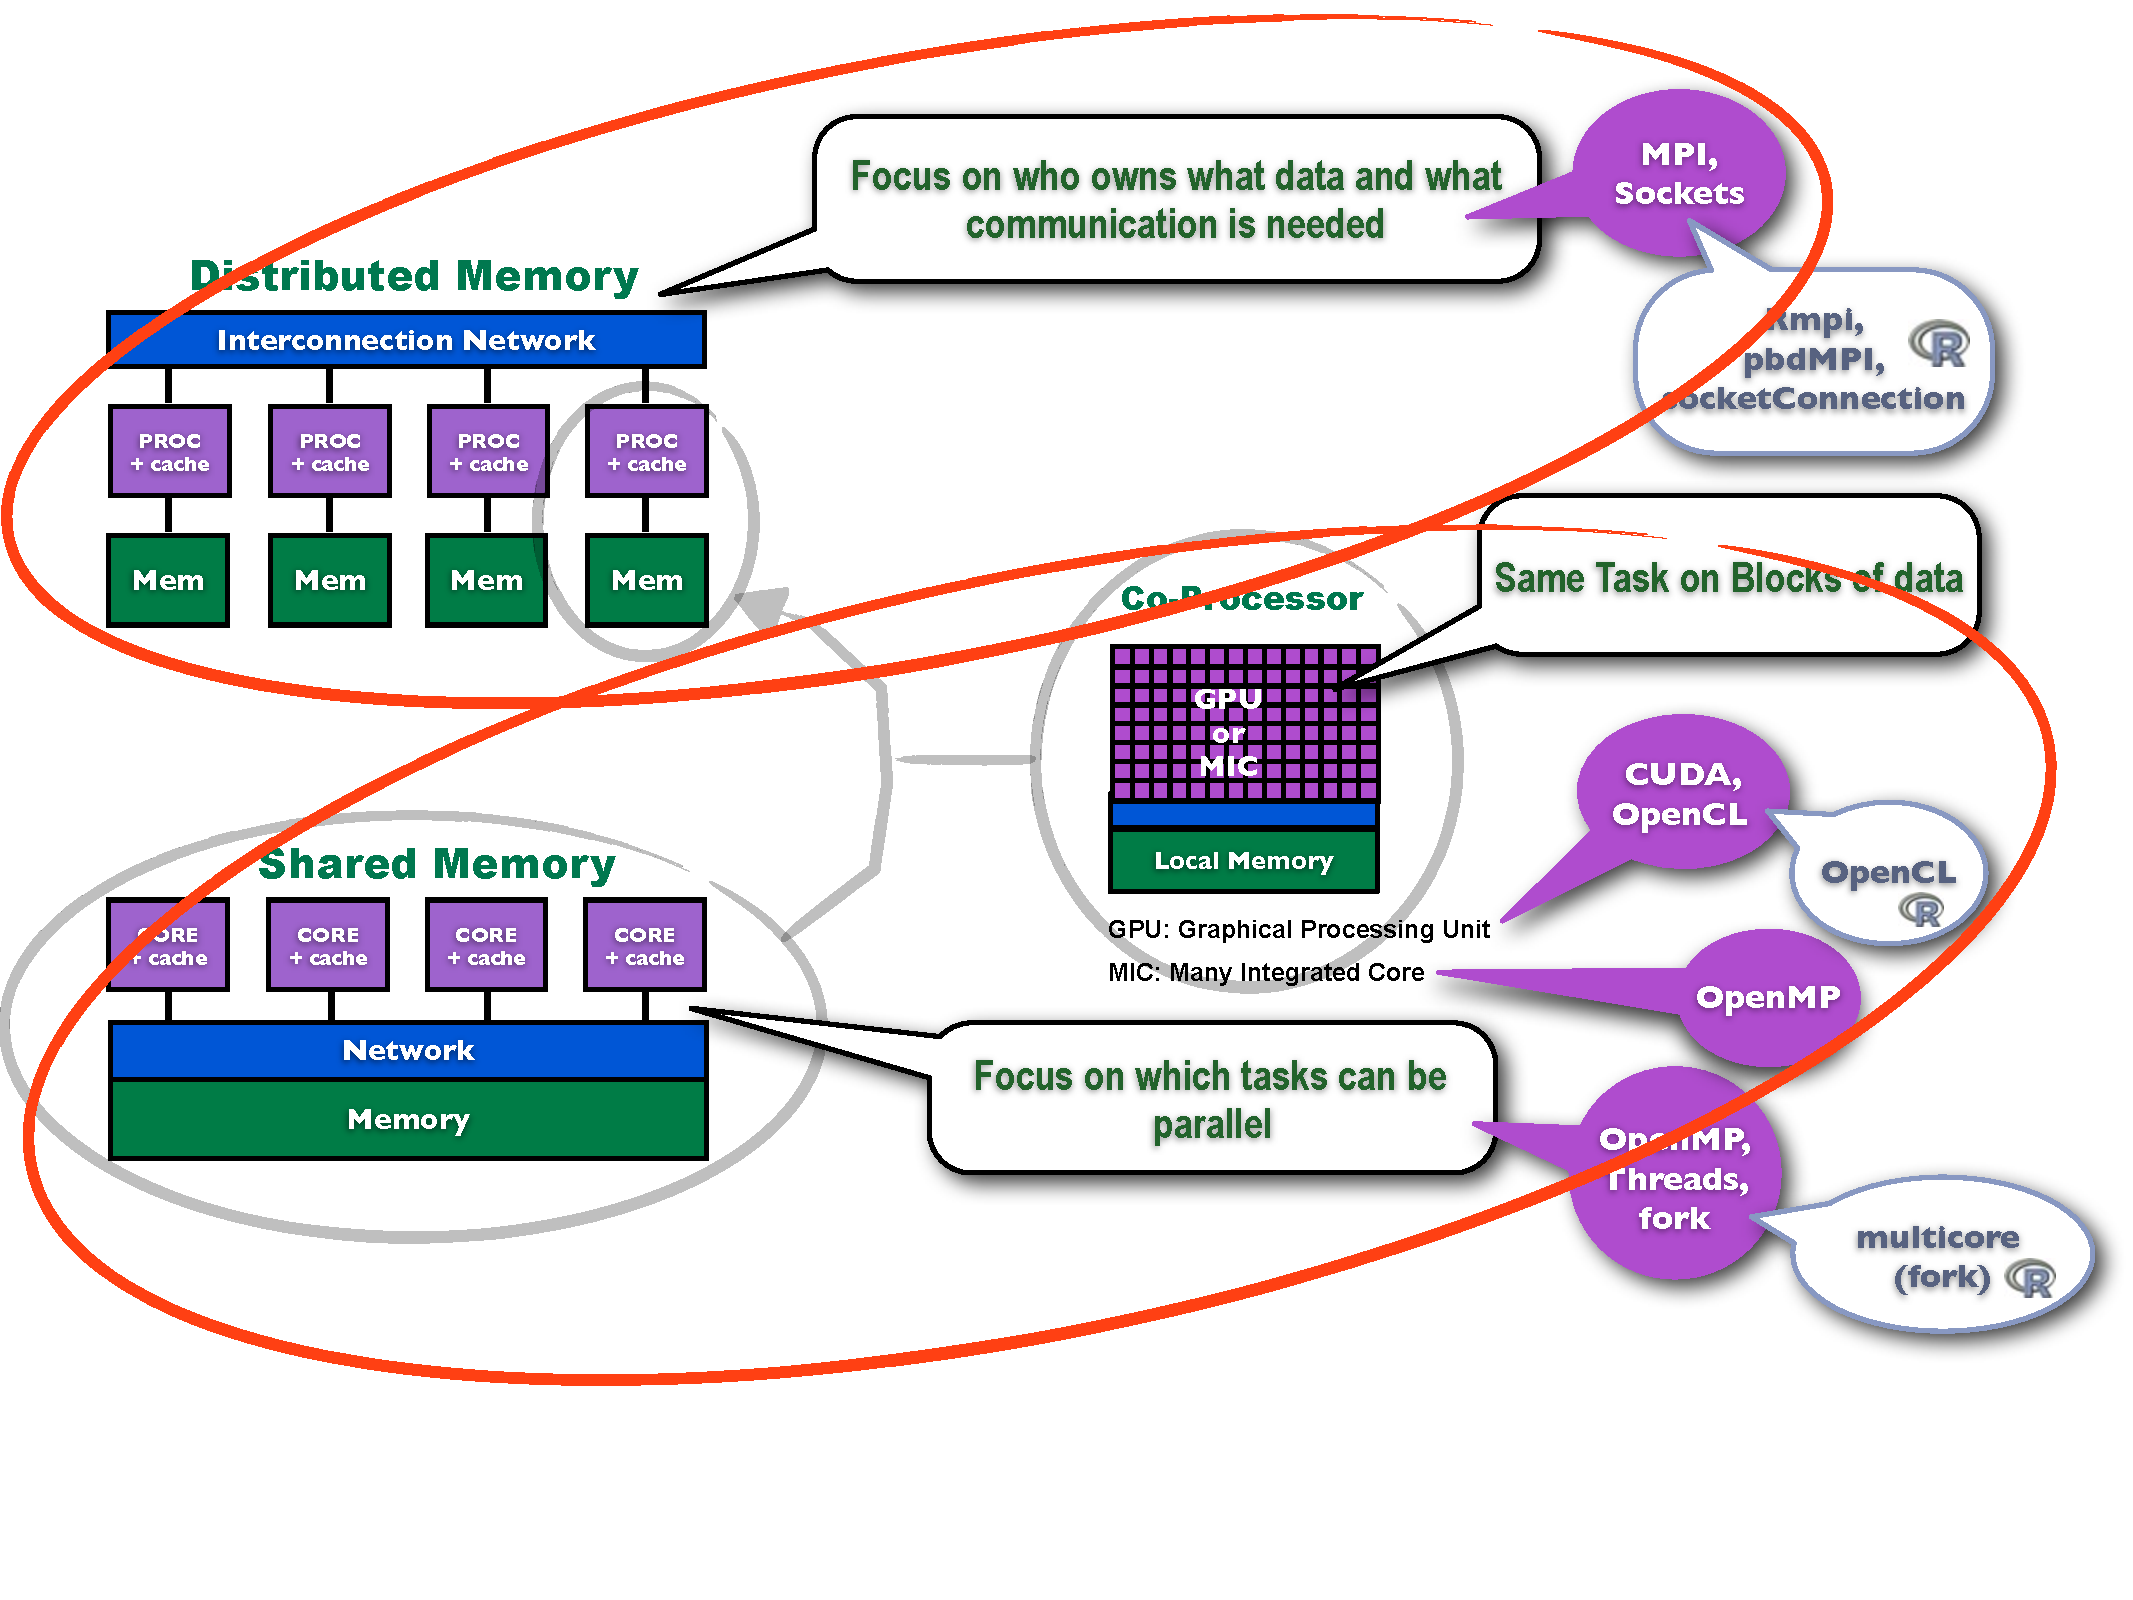
\includegraphics[height=\textheight]
{../common/pics/hardware/ParallelHardware10.pdf}
\end{frame}

\begin{frame}{HPC Libraries: 30+ Years of Research}
\includegraphics[height=\textheight]
{../common/pics/hardware/ParallelHardware25.pdf}
\end{frame}

\begin{frame}{R and \pbdR R Interfaces to HPC Libraries}
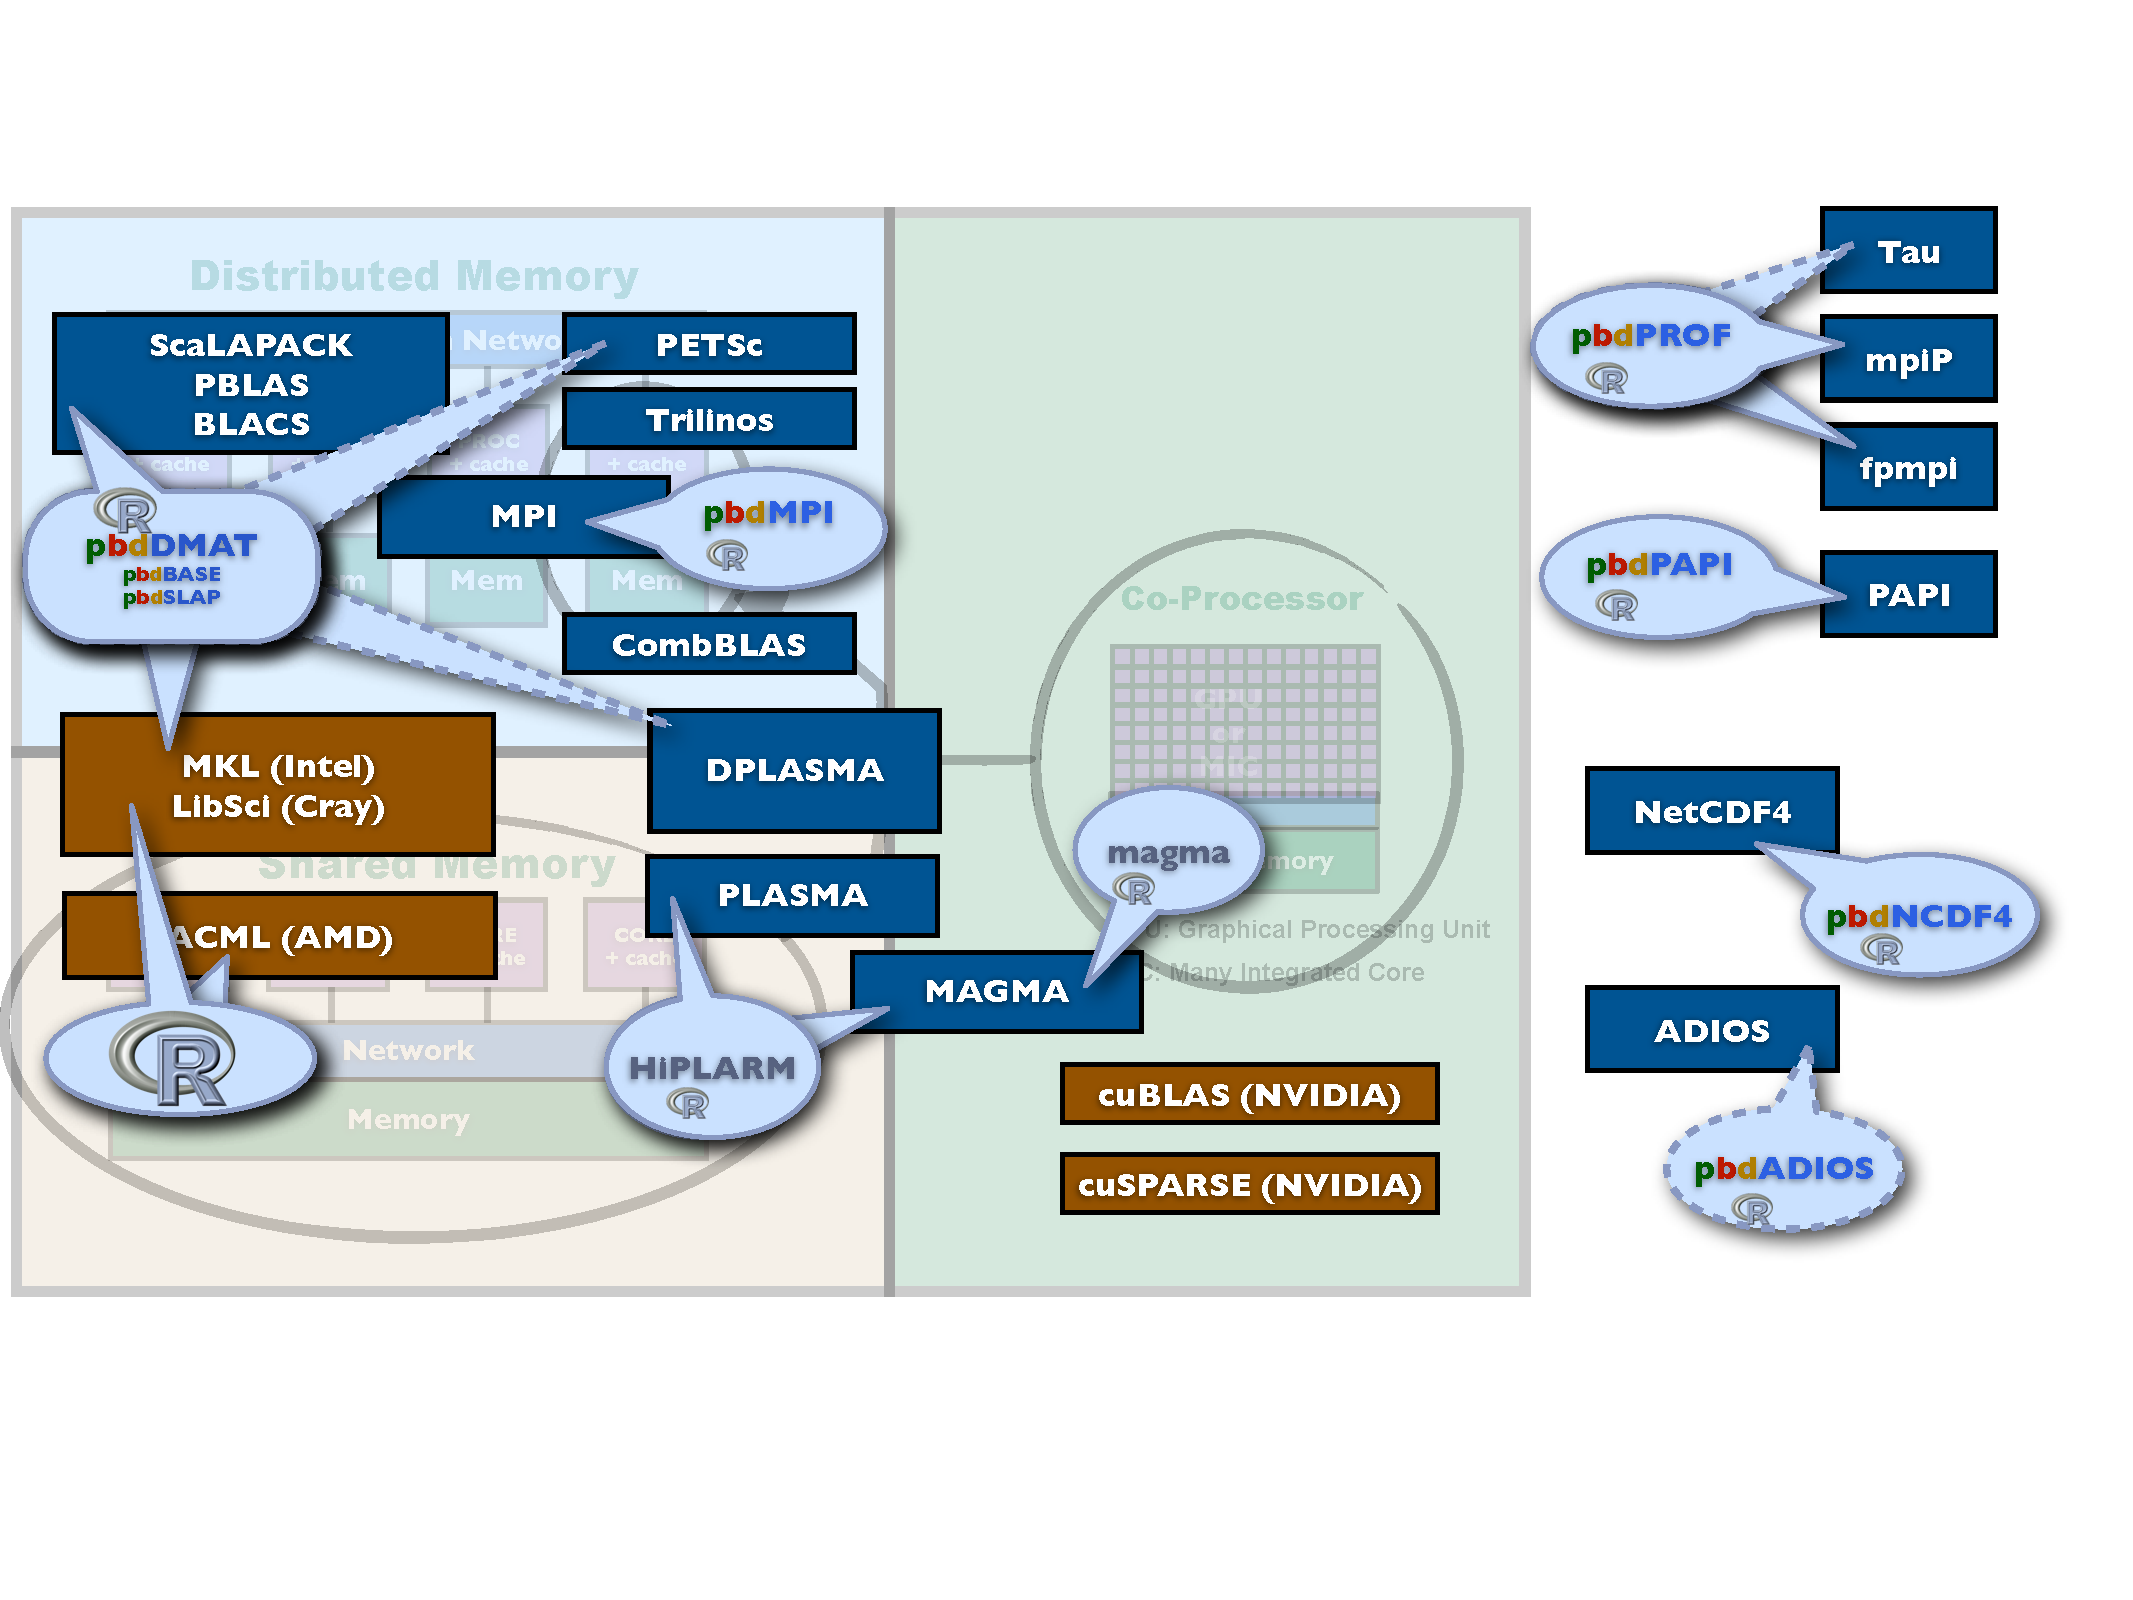
\includegraphics[height=\textheight]
{../common/pics/hardware/ParallelHardware26.pdf}
\end{frame}

\begin{frame}{Big Data and Little Data}
\begin{minipage}{10cm}
  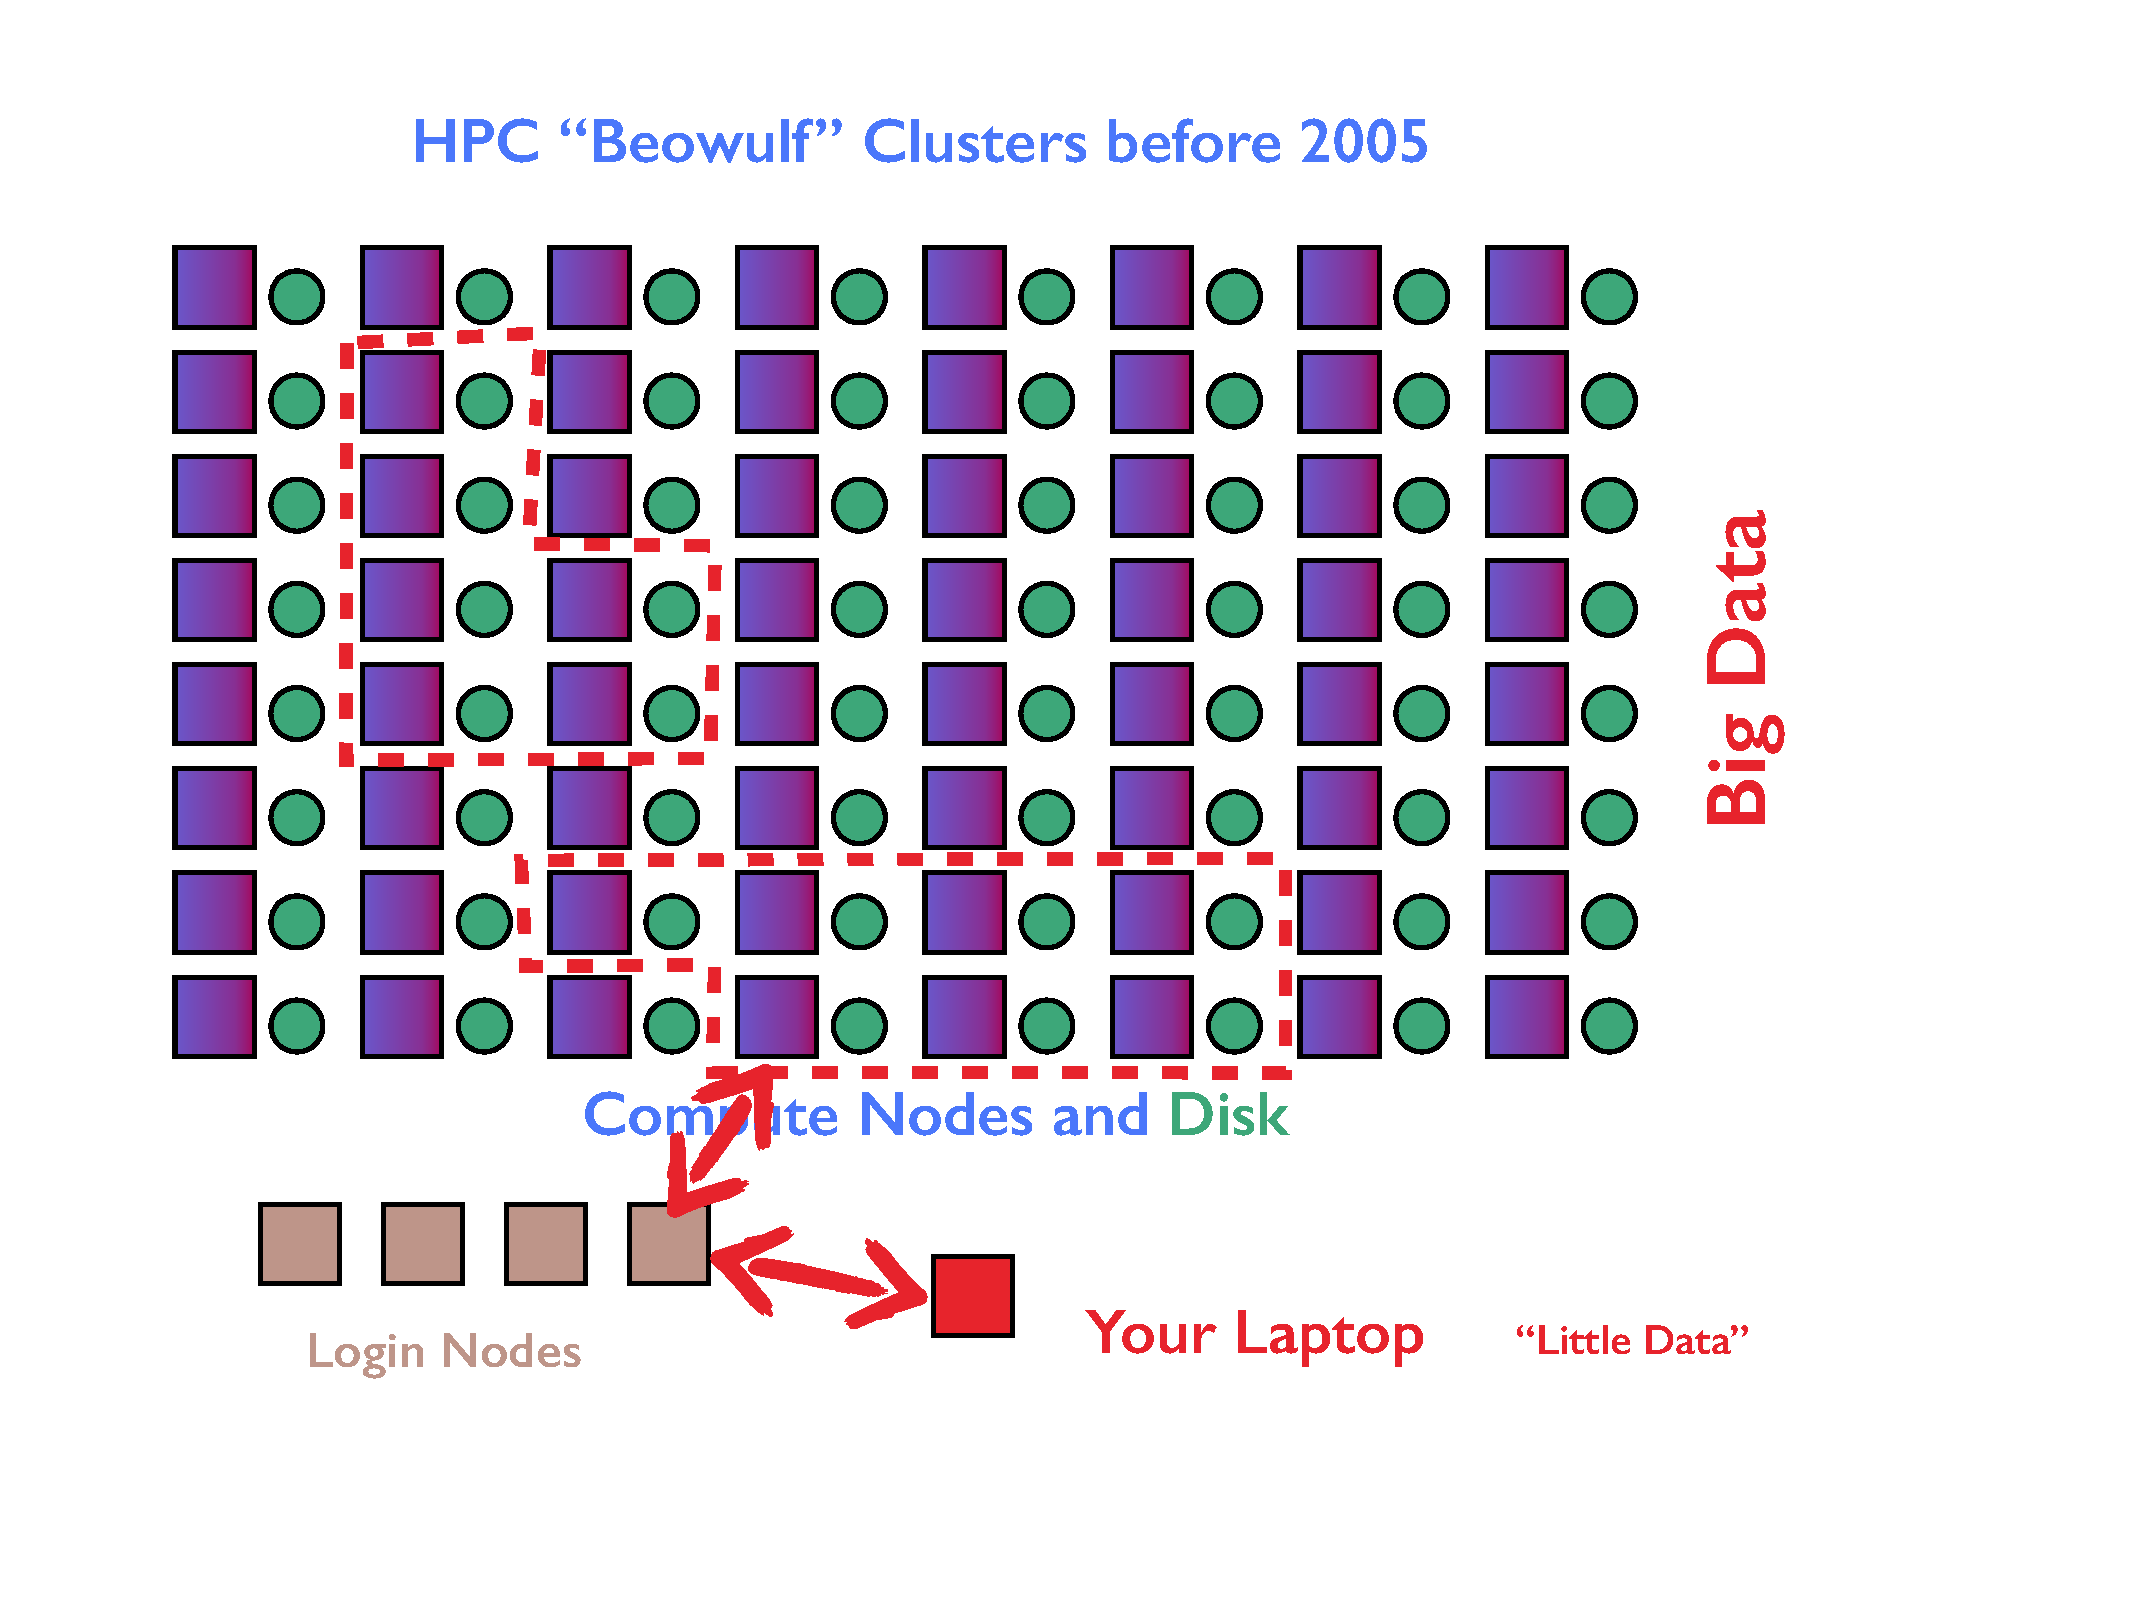
\includegraphics[height=0.9\textheight]
  {../common/pics/hardware/ParallelHardware22.pdf}\hfill
\end{minipage}
\begin{minipage}{5cm}\small
  \begin{block}{Analysis Workflow}\pause
    \begin{itemize}[<+-|alert@+>]
    \item Get Big Data
      \begin{itemize}
      \item Parallel data reader
      \item Parallel data generator
      \end{itemize}
    \item Write analysis script
    \item Graphics to display results
    \item Profile and optimize code
    \end{itemize}
  \end{block}
\end{minipage}
\end{frame}

\begin{frame}{Hadoop: Will it merge with HPC in the future?}
\begin{minipage}{8.5cm}
  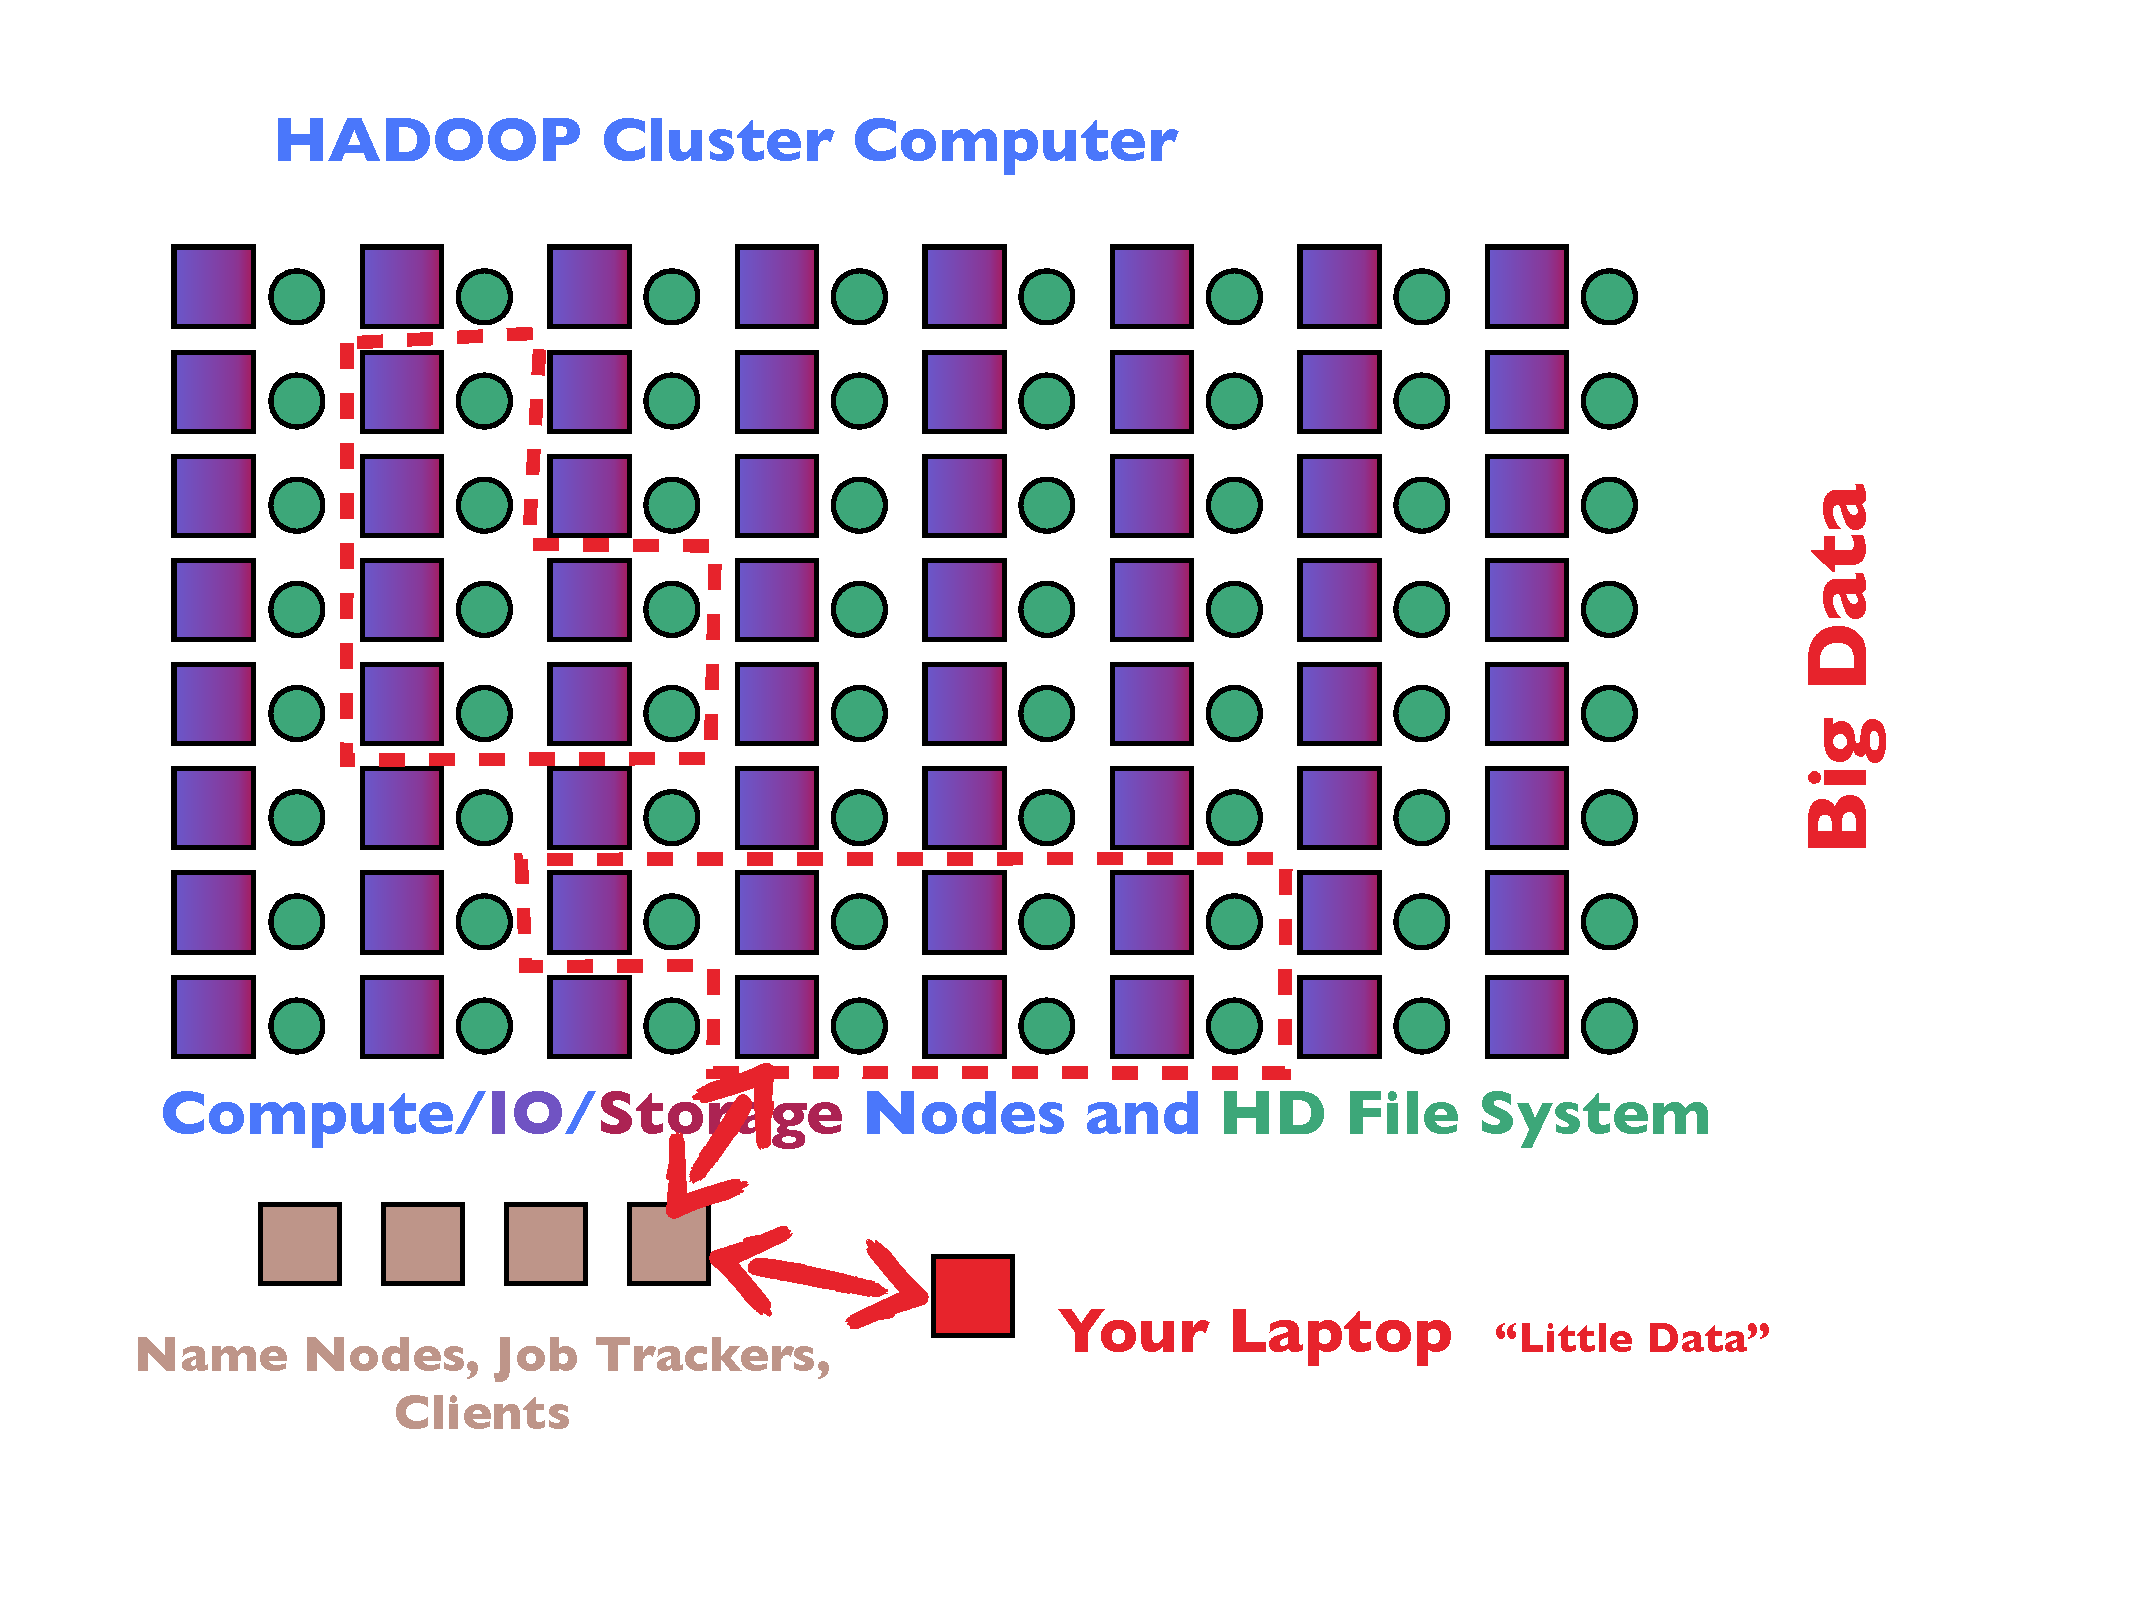
\includegraphics[trim=2cm 0cm 0cm 0cm,clip=true,height=0.8\textheight]
  {../common/pics/hardware/ParallelHardware23.pdf}
\end{minipage}
\begin{minipage}{3cm}\small
  \begin{block}{Components}\pause
%    \begin{itemize}[<+-|alert@+>]
    \scriptsize HDFS file system\\
    Yarn resource manager \\
    Map-reduce limitation
%    \end{itemize}
  \end{block}
\end{minipage}
\end{frame}

\begin{frame}{The future is here}
\includegraphics[height=0.9\textheight]
{../common/pics/hardware/ParallelHardware24.pdf}
\end{frame}

%\begin{frame}{\pbdR Interfaces to Libraries: Sustainable Path}
%\includegraphics[height=1.05\textheight]
%{../common/pics/hardware/ParallelHardware14.pdf}
%\end{frame}

%\begin{frame}{Low level R Interfaces to Native Tools}
%\includegraphics[width=0.95\textheight]
%{../common/pics/hardware/ParallelHardware22.pdf}
%\includegraphics[width=0.95\textheight]
%{../common/pics/hardware/ParallelHardware23.pdf}
%\end{frame}



\subsection{Batch and Interactive}
\makesubcontentsslidessec

\begin{frame}
  \begin{block}{Data analysis is interactive!}
    \pause
    \begin{itemize}[<+-|alert@+>]
    \item Data reduction to knowledge
    \item Iterative process with same data
      \begin{itemize}
      \item Exploration, model construction
      \item Diagnostics of fit and quantification of uncertainty
      \item Interpretation
      \end{itemize}
    \item S (and R) interactive ``answer'' to batch data analysis
    \item Efficient use of expensive people
    \end{itemize}
  \end{block}
  \begin{block}{Big platform computing is batch!}
    \pause
    \begin{itemize}[<+-|alert@+>]
    \item Libraries built for batch computing
    \item Traditionally data generation by simulation science
    \item Efficient use of expensive platforms
    \end{itemize}
  \end{block}
\end{frame}

\begin{frame}
  \begin{block}{High-Level Language: Batch and Interactive Distinction Blurred.}
    \begin{itemize}
    \item A function is a ``batch'' script
    \item \R ``An interactive environment to use batch scripts''
    \end{itemize}
  \end{block}
  \begin{block}{Ideal solution: Interactive Client with a Batch
      Server}
    \begin{itemize}
    \item Parallel visualization systems (VisIt and ParaView) are
      client-server (batch on server)
    \item Current \pbdR packages address server side (batch)
    \item pbdCS 0.1-0 released on GitHub
      \begin{itemize}
      \item Interactive SPMD
      \item Based on ZeroMQ distributed messaging (pbdZMQ 0.1-1 on CRAN)
      \item Bridge resource manager (pbdSCHED 0.1-0 on GitHub)
      \item Site configuration file
      \item Manage relationship of big data (server side) to little
        data (client side)
      \end{itemize}
    \end{itemize}
  \end{block}
\end{frame}


\subsection{Programming Models}
\makesubcontentsslidessec

\begin{frame}{Manager-Workers}
  \begin{block}{}
    \begin{itemize}
    \item A serial program (Manager) divides up work and/or data
    \item Workers run in parallel without interaction
    \item Manager collects/combines results from workers
    \item Divide-Recombine fits this model
    \end{itemize}
  \end{block}
\end{frame}

\begin{frame}{MapReduce}
  \begin{block}{}
    \begin{itemize}
    \item A concept born of a search engine
    \item Decouples certain coupled problems with an intermediate
      communication - shuffle
    \item User writes two serial codes: Map and Reduce
    \end{itemize}
  \end{block}
\end{frame}

\begin{frame}{MapReduce: a Parallel Search Engine Concept}
  \begin{block}{Search MANY documents \hfill Serve MANY users}
    \begin{center}\scriptsize
      \begin{equation*}
        \begin{array}{c@{\hspace{-2ex}}r@{\hspace{-2ex}}c}
          \begin{array}{c}
            \mbox{\scriptsize Web} \\
            \mbox{\scriptsize Pages} \\
            \mbox{\scriptsize (records)}
          \end{array} &
          \begin{array}{c}\tiny
            \\ \mbox{\tiny p0} \\ \mbox{\tiny p1} \\
            \mbox{\tiny p2} \\ \mbox{\tiny p3}
          \end{array} &
          \begin{array}{c}
            \mbox{\scriptsize Index Words (keys)} \\
            \left[
            \begin{array}{cccc}
              A_1 & A_2  & A_3 & A_4 \\
              \hline
              B_1 & B_2  & B_3 & B_4 \\
              \hline
              C_1 & C_2  & C_3 & C_4 \\
              \hline
              D_1 & D_2  & D_3 & D_4
            \end{array}
            \right]
          \end{array}
        \end{array}
        \hbox{\hspace{-2ex}}
        \begin{array}{c}
          \hbox{Shuffle} \\
          \longrightarrow \\
          \mbox{\code{MPI\_Alltoallv}}
        \end{array}
        \hbox{\hspace{-2ex}}
        \begin{array}{c@{\hspace{-2ex}}r@{\hspace{-2ex}}c}
          \begin{array}{c}
            \mbox{\scriptsize Index} \\
            \mbox{\scriptsize Words} \\
            \mbox{\scriptsize (keys)}
          \end{array} &
          \begin{array}{c}
            \\  \mbox{\tiny p0} \\ \mbox{\tiny p1} \\
            \mbox{\tiny p2} \\ \mbox{\tiny p3}
          \end{array} &
          \begin{array}{c}
            \mbox{\scriptsize Web Pages (records)} \\
            \left[
            \begin{array}{cccc}
              A_1 & B_1  & C_1 & D_1 \\
              \hline
              A_2 & B_2  & C_2 & D_2 \\
              \hline
              A_3 & B_3  & C_3 & D_3 \\
              \hline
              A_4 & B_4  & C_4 & D_4
            \end{array}
            \right]
          \end{array}
        \end{array}
      \end{equation*}
    \end{center}
    \vspace{2em}
    \begin{center}
      Matrix transpose in another language?
    \end{center}
  \end{block}
\end{frame}

\begin{frame}
  \begin{block}{Can use different sets of processors}
    \begin{center}
      \begin{equation*}\scriptsize
        \begin{array}{c@{\hspace{-2ex}}r@{\hspace{-2ex}}c}
          \begin{array}{c}
            \mbox{\scriptsize Web} \\
            \mbox{\scriptsize Pages} \\
            \mbox{\scriptsize (records)}
          \end{array} &
          \begin{array}{c}\tiny
            \\ \mbox{\tiny p0} \\ \mbox{\tiny p1} \\
            \mbox{\tiny p2} \\ \mbox{\tiny p3}
          \end{array} &
          \begin{array}{c}
            \mbox{\scriptsize Index Words (keys)} \\
            \left[
            \begin{array}{cccc}
              \\
              \hline
              B_1 & B_2  & B_3 & B_4 \\
              \hline
              \\
              \hline
              \\
            \end{array}
            \right]
          \end{array}
        \end{array}
        \hbox{\hspace{-2ex}}
        \begin{array}{c}
          \hbox{Streaming} \\
          \hbox{Shuffle} \\
          \longrightarrow \\
          \mbox{\code{MPI\_Scatter}}
        \end{array}
        \hbox{\hspace{-2ex}}
        \begin{array}{c@{\hspace{-2ex}}r@{\hspace{-2ex}}c}
          \begin{array}{c}
            \mbox{\scriptsize Index} \\
            \mbox{\scriptsize Words} \\
            \mbox{\scriptsize (keys)}
          \end{array} &
          \begin{array}{c}
            \\  \mbox{\tiny p4} \\ \mbox{\tiny p5} \\
            \mbox{\tiny p6} \\ \mbox{\tiny p7}
          \end{array} &
          \begin{array}{c}
            \mbox{\scriptsize Web Pages (records)} \\
            \left[
            \begin{array}{cccc}
              \quad  & B_1  & \quad & \quad \\
              \hline
              \quad  & B_2  & \quad  &  \quad \\
              \hline
              \quad  & B_3  & \quad  &  \quad \\
              \hline
              \quad  & B_4  & \quad  & \quad
            \end{array}
            \right]
          \end{array}
        \end{array}
      \end{equation*}
    \end{center}
  \end{block}
\end{frame}

\begin{frame}{MPI and MapReduce}
  \begin{block}{Both Concepts are about Communitation}
    \begin{itemize}
    \item One makes communication explicit, gives choices
    \item The other hides communication, gives one choice (shuffle)
    \end{itemize}
  \end{block}
\end{frame}

\begin{frame}{SPMD: Single Program Multiple Data}
  \begin{block}{}
    \begin{itemize}
    \item The prevalent way of distributed programming
    \item Can handle tightly coupled parallel computations
    \item It is designed for batch computing
    \item There is usually no manager - rather, all cooperate
    \item Prime driver behind MPI specification
    \end{itemize}
  \end{block}
\end{frame}

\begin{frame}{Early SPMD Work in Statistics: Crossproduct (Row-Block)}
  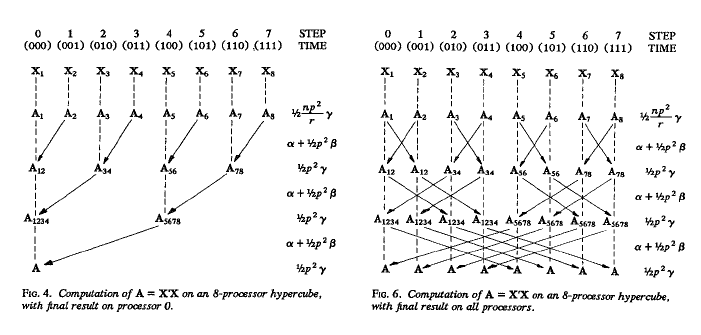
\includegraphics[width=\textwidth]
  {../common/pics/comm/Crossprod1987.png} \\
  \begin{block}{Hypercube: Individual send() and recv() over each dimension}
    {\scriptsize Ostrouchov (1987). Parallel Computing on a
      Hypercube: An overview of the architecture and some
      applications. {\em Proceedings of the 19th Symposium on the
        Interface of Computer Science and Statistics}, p.27-32.}
  \end{block}
\end{frame}

\begin{frame}{Simplified with MPI (and further with pbdMPI)}
  \includegraphics[trim=0cm 6cm 0cm 4cm,clip=true,width=\textwidth]
  {../common/pics/comm/ParallelHardware30.pdf}
  \vspace{-1ex}
  \begin{block}{Architecture-specific vendor optimizations}
    \begin{itemize}
    \item \small Cray MPT
    \item \small SGI MPT
    \end{itemize}
  \end{block}
\end{frame}

\begin{frame}{Data-flow: Parallel Runtime Scheduling and Execution
    Controller (PaRSEC)}
  \vspace{-.1cm}
  \hspace{2cm}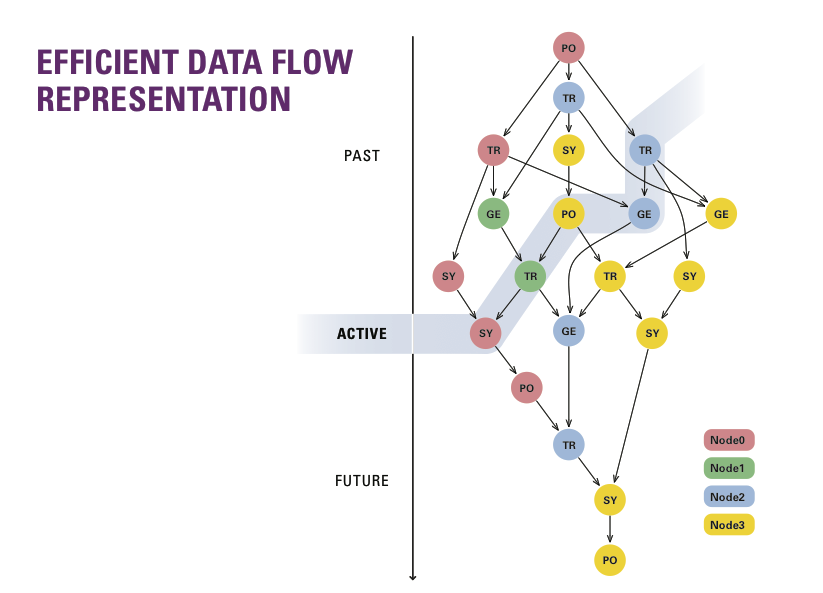
\includegraphics[trim=0cm 0cm 0cm
  1cm,clip=true,width=7.5cm]{../common/pics/comm/PaRSEC1.png}
 \\[-3.4cm]
  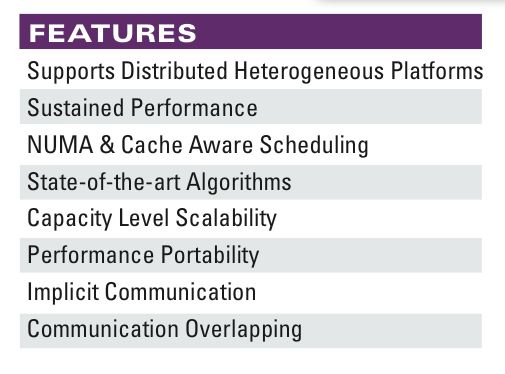
\includegraphics[width=4cm]{../common/pics/comm/PaRSEC2.png}
  \hspace{5cm}{\tiny Graphic from icl.cs.utk.edu}
  \begin{block}
    {\tiny Bosilca, G., Bouteiller, A., Danalis, A., Faverge,
      M., Herault, T., Dongarra, J. "PaRSEC: Exploiting Heterogeneity
      to Enhance Scalability," IEEE Computing in Science and
      Engineering, Vol. 15, No. 6, 36-45, November, 2013.}
    \begin{itemize}\small
    \item Master data-flow controller runs distributed on all cores.
    \item Dynamic generation of current level in flow graph
    \item Effectively removes collective synchronizations
    \end{itemize}
  \end{block}
\end{frame}

\section{pbdR}
\makesubcontentsslides

\subsection{The pbdR Project}
\makesubcontentsslidessec

\begin{frame}{\pbdR Interfaces to Libraries: Sustainable Path}
  \vspace{-1ex}
  \centering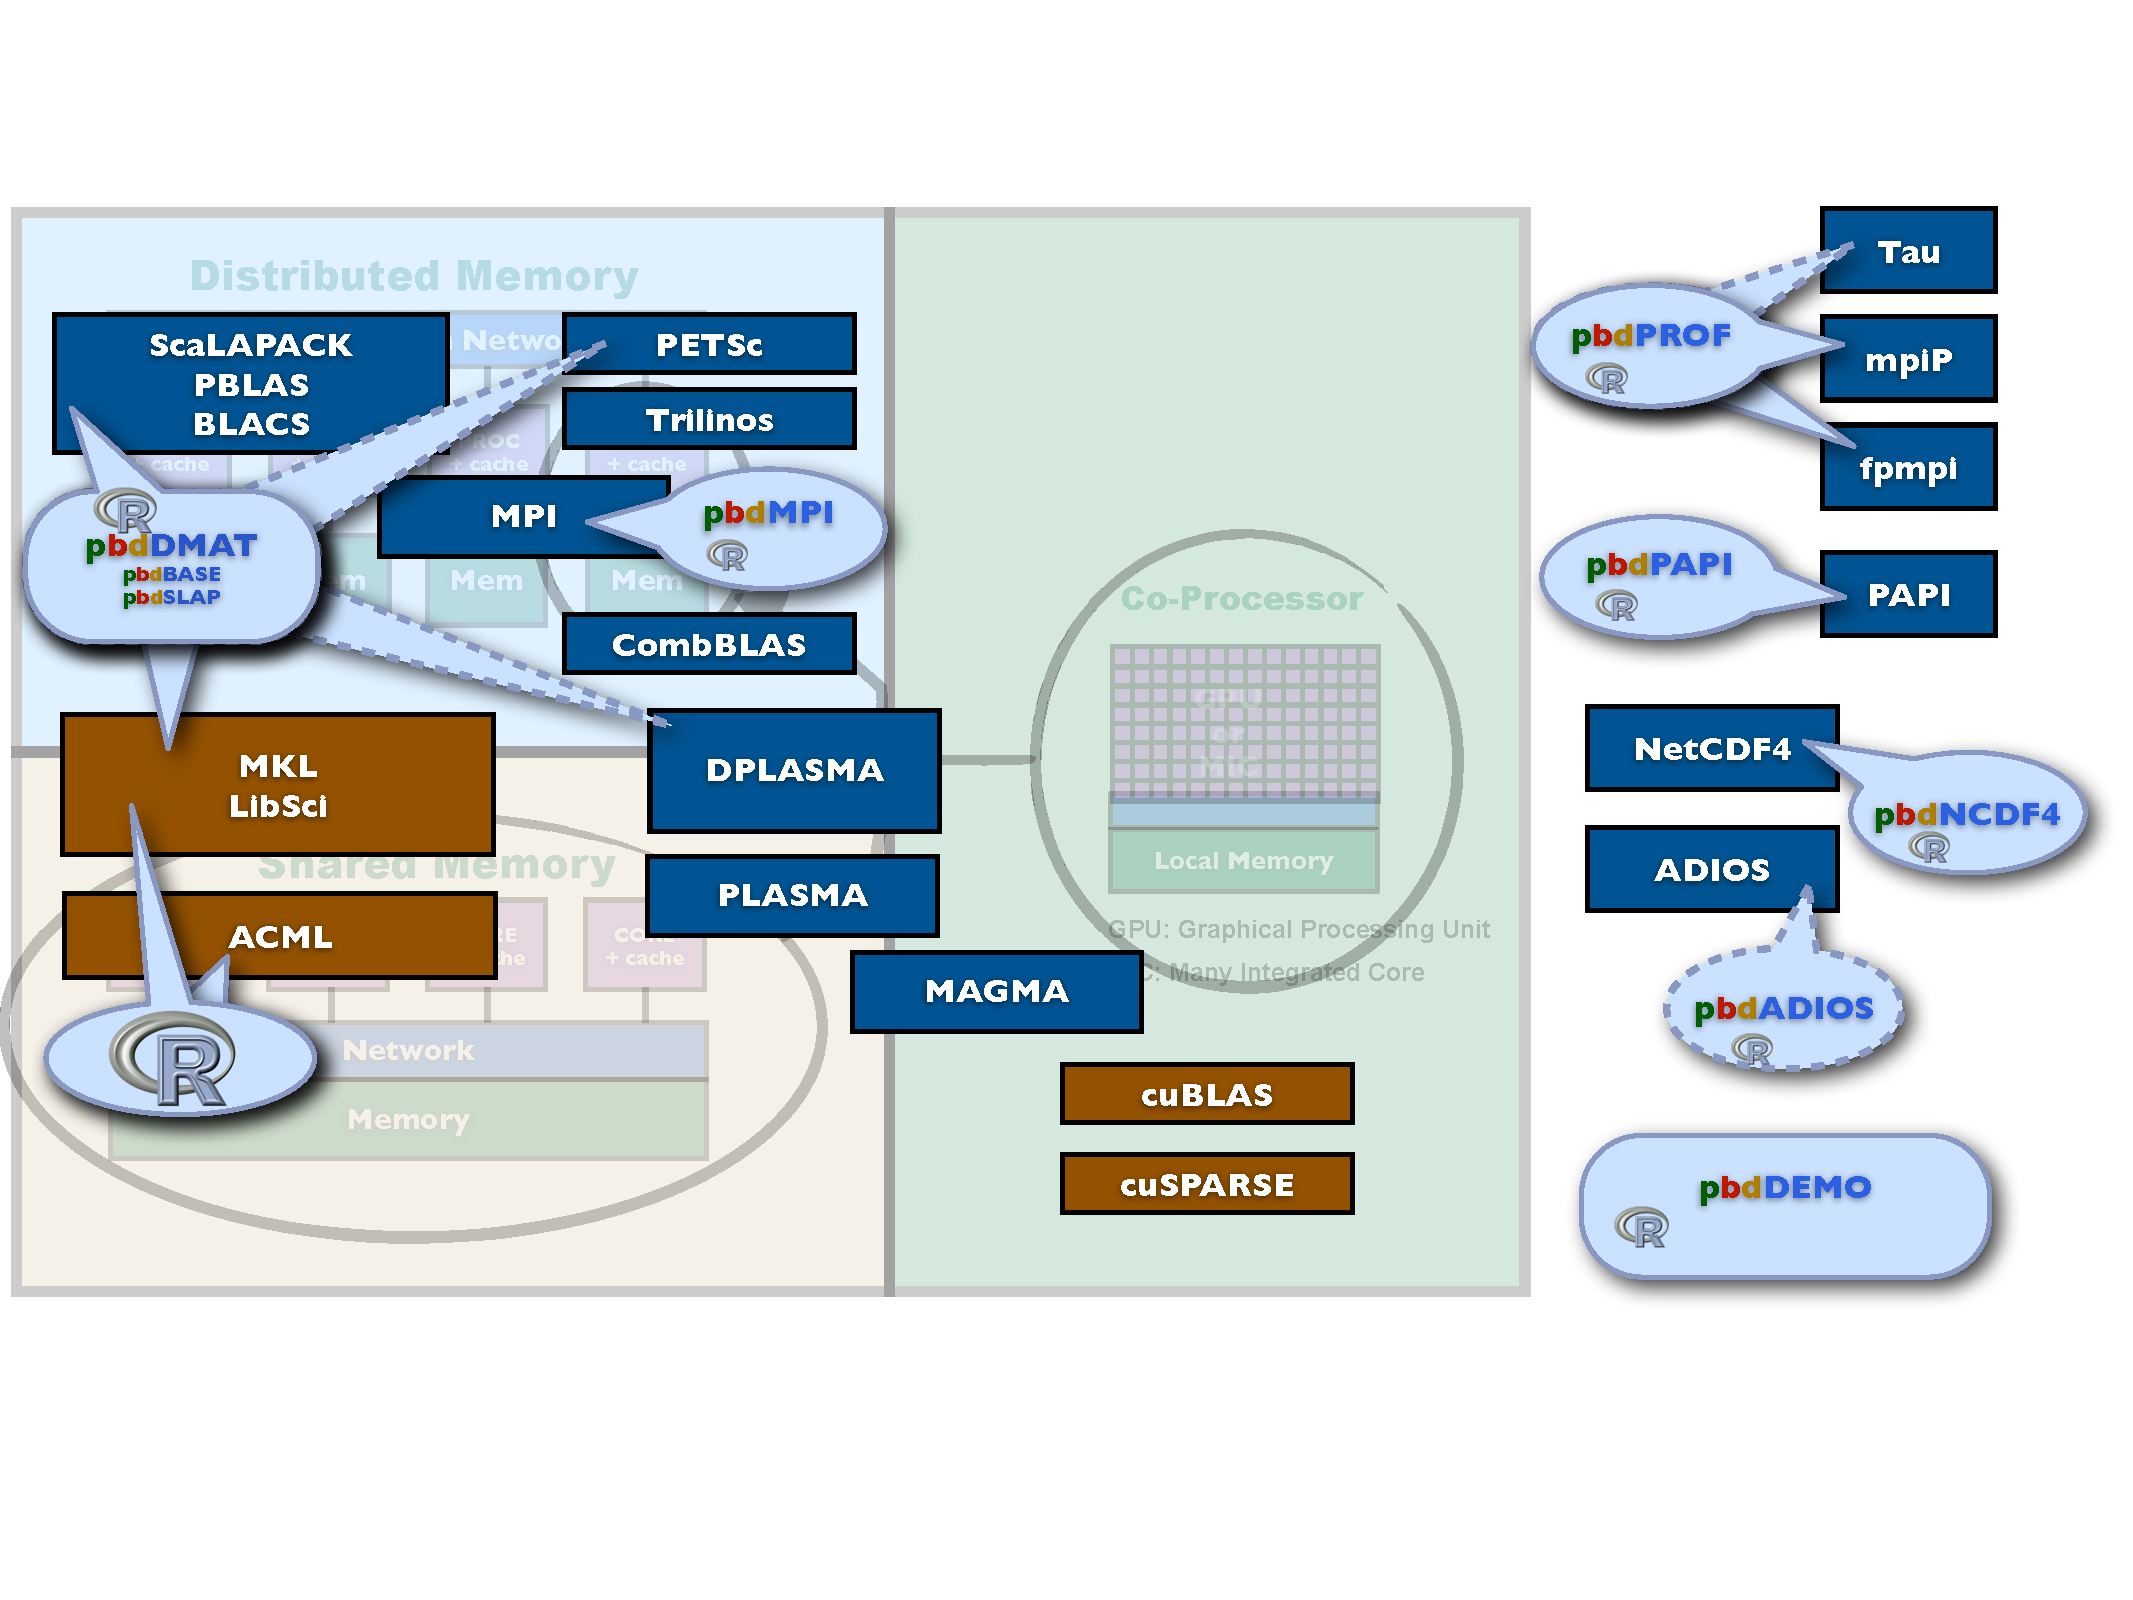
\includegraphics[trim=0cm 5cm 0cm 3cm,clip=true,width=0.85\textwidth]
  {../common/pics/hardware/ParallelHardware27.pdf}
  \scriptsize
  \begin{block}{Why use HPC libraries?}
    \begin{itemize}[<+-|alert@+>]
    \item The HPC community is 30 years beyond ``embarrassingly parallel.''
    \item \emph{They're tested.} \emph{They're
        fast.}  \emph{They're scalable.}
    \item Many science communities are invested in their API.
    \item Data analysis uses much of the same math as simulation science.
    \end{itemize}
  \end{block}
\end{frame}

\subsection{pbdMPI}
\makesubcontentsslidessec

\begin{frame}
  \begin{block}{pbdMPI: a High Level Interface to MPI}
    \begin{itemize}
    \item API is simplified: defaults in control objects.
    \item S4 methods: extensible to complex \R objects.
    \item Additional error checking
    \item Array and matrix methods without serialization: faster than
      \pkg{Rmpi}.
    \end{itemize}
    \begin{center}
      \vspace{0.2cm}\scriptsize
      \begin{tabular}{ll} \hline\hline
        \pkg{pbdMPI} (S4) & \pkg{Rmpi}                \\ \hline
        \code{\color{blue}allreduce}    & \code{mpi.allreduce}      \\
        \code{\color{blue}allgather}    & \code{mpi.allgather},
        \code{mpi.allgatherv},
        \code{mpi.allgather.Robj} \\
        \code{bcast}        & \code{mpi.bcast},
        \code{mpi.bcast.Robj}     \\
        \code{gather}       & \code{mpi.gather},
        \code{mpi.gatherv},
        \code{mpi.gather.Robj}    \\
        \code{recv}         & \code{mpi.recv},
        \code{mpi.recv.Robj}      \\
        \code{reduce}       & \code{mpi.reduce}         \\
        \code{scatter}      & \code{mpi.scatter},
        \code{mpi.scatterv},
        \code{mpi.scatter.Robj}   \\
        \code{send}         & \code{mpi.send},
        \code{mpi.send.Robj}      \\ \hline \hline
      \end{tabular}
    \end{center}
  \end{block}
\end{frame}

\begin{frame}[fragile]
  \begin{block}{Integer?\qquad Not always obvious in R.}
    \vspace{-.2cm}
    \begin{lstlisting}
> is.integer(1)
[1] FALSE
> is.integer(2)
[1] FALSE
> is.integer(1:2)
[1] TRUE
    \end{lstlisting}
  \end{block}
  \begin{block}{Often it's best to let the machine figure it out}\pause
    \begin{minipage}[t]{.475\textwidth}
      \begin{lstlisting}[title=Rmpi]
# int
mpi.allreduce(x, type=1)
# double
mpi.allreduce(x, type=2)
      \end{lstlisting}
    \end{minipage}
    \hfill
    \begin{minipage}[t]{.475\textwidth}
      \begin{lstlisting}[title=pbdMPI]
allreduce(x)
      \end{lstlisting}
      % \vspace{1em}
      % \hspace{1em}{\small S4. Batch only! (No spawning)}
    \end{minipage}
  \end{block}
\end{frame}



% \begin{frame}[fragile,shrink]
%   \begin{block}{Embarrassingly Parallel Computation}\pause
%     \vspace{-1ex}
%     \begin{minipage}[t]{.45\textwidth}
%       \begin{lstlisting}[title=EPforeach.R "asking for parallel",basicstyle=\tiny]
% library(doMPI, quiet=TRUE)
% cl <- startMPIcluster()
% registerDoMPI(cl)

% n <- 10
% myIn <- vector("list", n)

% myFun <- function(x) {
%   s <- sum(rnorm(10000))
%   rank <- mpi.comm.rank(comm=0)
%   return(paste(s, "from", rank))
% }

% results <- foreach(i = 1:n) %dopar% {
%   out <- myFun(myIn[[i]])
% }

% print(results)

% closeCluster(cl)
% mpi.quit()
%       \end{lstlisting}
%     \end{minipage}
%     \hfill
%     \begin{minipage}[t]{.5\textwidth}
%       \begin{lstlisting}[title=EPpbdR.R "thinking parallel",basicstyle=\tiny]
% library(pbdMPI, quiet=TRUE)
% init()

% myChunk <- get.jid(n <- 10)
% myIn <- vector("list", length(myChunk))
% myOut <- vector("list", length(myChunk))

% myFun = function(x) {
%   s <- sum(rnorm(10000))
%   rank <- comm.rank()
%   return(paste(s, "from", rank))
% }

% for(i in 1:length(myChunk)) {
%   myOut[[i]] <- myFun(myIn[[i]])
% }
% results <- gather(myOut)

% comm.print(results)
% finalize()
%       \end{lstlisting}
%     \end{minipage}
%   \end{block}
% \end{frame}


\begin{frame}[fragile]{SPMD Runs Many Copies of One Code}
  \begin{exampleblock}{SPMD Hello World: a ``map-reduce'' to all}
    \vspace{-1.5ex}
    \centering
    \begin{lstlisting}[title=map-reduce.r]
library(pbdMPI, quiet = TRUE)
init()

## Your "Map" code
n <- comm.rank() + 1

## Now "Reduce" but give the result to all
all_sum <- allreduce(n) # Sum is default

text <- paste("Hello: n is", n, "sum is", all_sum )
comm.print(text, all.rank=TRUE)

finalize()
    \end{lstlisting}
    \vspace{-4.5ex}
    \begin{columns}[t,onlytextwidth]
      \begin{column}{0.54\textwidth}
        \begin{lstlisting}[backgroundcolor=\color{white},keywordstyle=\color{black},
title=Execute this batch script via:]
mpirun -np 2 Rscript map-reduce.r
        \end{lstlisting}
      \end{column}
      \hfill
      \begin{column}{0.46\textwidth}
        \begin{lstlisting}[title=Output:]
COMM.RANK = 0
[1] "Hello: n is 1 sum is 3"
COMM.RANK = 1
[1] "Hello: n is 2 sum is 3"
        \end{lstlisting}
      \end{column}
    \end{columns}
  \end{exampleblock}
\end{frame}

\subsection{pbdDMAT}
\makesubcontentsslidessec

\begin{frame}{Dense Matrix and Vector Operations}
  \begin{block}{A matrix is mapped to a processor grid shape}
    \begin{table}[ht]
      \centering
      % \begin{subfigure}[b]{0.23\textwidth}
      %   \centering
      %   $\left[\begin{tabular}{l}
      %       0 \\ 1 \\ 2 \\ 3 \\ 4 \\ 5
      %     \end{tabular}\right]^T$
      %   \caption{$1\times 6$}
      % \end{subfigure}
      \begin{subfigure}[b]{0.23\textwidth}
        \centering
        $\left[\begin{tabular}{llllll}
            0 & 1 & 2 & 3 & 4 & 5
          \end{tabular}\right]$
        \vspace{1.5cm}
        \caption{$1\times 6$}
      \end{subfigure}%\hspace{-1cm}
      \begin{subfigure}[b]{0.23\textwidth}
        \centering
        $\left[\begin{tabular}{lll}
            0 & 1 & 2\\
            3 & 4 & 5
          \end{tabular}\right]$
        \caption{$2\times 3$}
      \end{subfigure}%
      \begin{subfigure}[b]{0.23\textwidth}
        \centering
        $\left[\begin{tabular}{ll}
            0 & 1 \\
            2 & 3\\
            4 & 5
          \end{tabular}\right]$
        \caption{$3\times 2$}
      \end{subfigure}
      \begin{subfigure}[b]{0.23\textwidth}
        \centering
        $\left[\begin{tabular}{l}
            0 \\ 1 \\ 2 \\ 3 \\ 4 \\ 5
          \end{tabular}\right]$
        \caption{$6\times 1$}
      \end{subfigure}
      \caption{Processor Grid Shapes with 6 Processors}\label{fig:gridshapes}
    \end{table}
  \end{block}
\end{frame}

\begin{frame}[shrink]
\begin{exampleblock}{2$\times$3 block-cyclic grid on 6 processors:
    Global view ``ddmatrix'' class}
\begin{align*}
x &= \left[
      \begin{array}{ll|ll|ll|ll|l}
      \color{g11}x_{11} & \color{g11}x_{12} & \color{g12}x_{13} & \color{g12}x_{14} & \color{g13}x_{15} & \color{g13}x_{16} & \color{g11}x_{17} & \color{g11}x_{18} & \color{g12}x_{19}\\
      \color{g11}x_{21} & \color{g11}x_{22} & \color{g12}x_{23} & \color{g12}x_{24} & \color{g13}x_{25} & \color{g13}x_{26} & \color{g11}x_{27} & \color{g11}x_{28} & \color{g12}x_{29}\\\hline
      \color{g21}x_{31} & \color{g21}x_{32} & \color{g22}x_{33} & \color{g22}x_{34} & \color{g23}x_{35} & \color{g23}x_{36} & \color{g21}x_{37} & \color{g21}x_{38} & \color{g22}x_{39}\\
      \color{g21}x_{41} & \color{g21}x_{42} & \color{g22}x_{43} & \color{g22}x_{44} & \color{g23}x_{45} & \color{g23}x_{46} & \color{g21}x_{47} & \color{g21}x_{48} & \color{g22}x_{49}\\\hline
      \color{g11}x_{51} & \color{g11}x_{52} & \color{g12}x_{53} & \color{g12}x_{54} & \color{g13}x_{55} & \color{g13}x_{56} & \color{g11}x_{57} & \color{g11}x_{58} & \color{g12}x_{59}\\
      \color{g11}x_{61} & \color{g11}x_{62} & \color{g12}x_{63} & \color{g12}x_{64} & \color{g13}x_{65} & \color{g13}x_{66} & \color{g11}x_{67} & \color{g11}x_{68} & \color{g12}x_{69}\\\hline
      \color{g21}x_{71} & \color{g21}x_{72} & \color{g22}x_{73} & \color{g22}x_{74} & \color{g23}x_{75} & \color{g23}x_{76} & \color{g21}x_{77} & \color{g21}x_{78} & \color{g22}x_{79}\\
      \color{g21}x_{81} & \color{g21}x_{82} & \color{g22}x_{83} & \color{g22}x_{84} & \color{g23}x_{85} & \color{g23}x_{86} & \color{g21}x_{87} & \color{g21}x_{88} & \color{g22}x_{89}\\\hline
      \color{g11}x_{91} & \color{g11}x_{92} & \color{g12}x_{93} & \color{g12}x_{94} & \color{g13}x_{95} & \color{g13}x_{96} & \color{g11}x_{97} & \color{g11}x_{98} & \color{g12}x_{99}\\
      \end{array}
\right]_{9\times 9}
\end{align*}
\begin{align*}
\text{Processor grid = }\left|
      \begin{array}{lll}
      \color{g11}0 & \color{g12}1 & \color{g13}2\\
      \color{g21}3 & \color{g22}4 & \color{g23}5
      \end{array}
\right| &=
\left|
      \begin{tabular}{lll}
      \color{g11}(0,0) & \color{g12}(0,1) & \color{g13}(0,2)\\
      \color{g21}(1,0) & \color{g22}(1,1) & \color{g23}(1,2)
      \end{tabular}
\right|
\end{align*}
\end{exampleblock}
\end{frame}


\begin{frame}[shrink]
\begin{exampleblock}{2$\times$3 block-cyclic grid on 6 processors:
    Local view ``ddmatrix'' class}
\begin{align*}
\left[
      \begin{array}{ll|ll}
      \color{g11}x_{11} & \color{g11}x_{12} & \color{g11}x_{17} & \color{g11}x_{18}\\
      \color{g11}x_{21} & \color{g11}x_{22} & \color{g11}x_{27} & \color{g11}x_{28}\\\hline
      \color{g11}x_{51} & \color{g11}x_{52} & \color{g11}x_{57} & \color{g11}x_{58}\\
      \color{g11}x_{61} & \color{g11}x_{62} & \color{g11}x_{67} & \color{g11}x_{68}\\\hline
      \color{g11}x_{91} & \color{g11}x_{92} & \color{g11}x_{97} & \color{g11}x_{98}\\
      \end{array}
\right]_{5\times 4}
\left[
      \begin{array}{ll|l}
      \color{g12}x_{13} & \color{g12}x_{14} & \color{g12}x_{19}\\
      \color{g12}x_{23} & \color{g12}x_{24} & \color{g12}x_{29}\\\hline
      \color{g12}x_{53} & \color{g12}x_{54} & \color{g12}x_{59}\\
      \color{g12}x_{63} & \color{g12}x_{64} & \color{g12}x_{69}\\\hline
      \color{g12}x_{93} & \color{g12}x_{94} & \color{g12}x_{99}\\
      \end{array}
\right]_{5\times 3}
\left[
      \begin{array}{ll}
      \color{g13}x_{15} & \color{g13}x_{16}\\
      \color{g13}x_{25} & \color{g13}x_{26}\\\hline
      \color{g13}x_{55} & \color{g13}x_{56}\\
      \color{g13}x_{65} & \color{g13}x_{66}\\\hline
      \color{g13}x_{95} & \color{g13}x_{96}\\
      \end{array}
\right]_{5\times 2}
\\
\left[
      \begin{array}{ll|ll}
      \color{g21}x_{31} & \color{g21}x_{32} & \color{g21}x_{37} & \color{g21}x_{38}\\
      \color{g21}x_{41} & \color{g21}x_{42} & \color{g21}x_{47} & \color{g21}x_{48}\\\hline
      \color{g21}x_{71} & \color{g21}x_{72} & \color{g21}x_{77} & \color{g21}x_{78}\\
      \color{g21}x_{81} & \color{g21}x_{82} & \color{g21}x_{87} & \color{g21}x_{88}\\
      \end{array}
\right]_{4\times 4}
\left[
      \begin{array}{ll|l}
      \color{g22}x_{33} & \color{g22}x_{34} & \color{g22}x_{39}\\
      \color{g22}x_{43} & \color{g22}x_{44} & \color{g22}x_{49}\\\hline
      \color{g22}x_{73} & \color{g22}x_{74} & \color{g22}x_{79}\\
      \color{g22}x_{83} & \color{g22}x_{84} & \color{g22}x_{89}\\
      \end{array}
\right]_{4\times 3}
\left[
      \begin{array}{ll}
      \color{g23}x_{35} & \color{g23}x_{36} \\
      \color{g23}x_{45} & \color{g23}x_{46} \\\hline
      \color{g23}x_{75} & \color{g23}x_{76} \\
      \color{g23}x_{85} & \color{g23}x_{86} \\
      \end{array}
\right]_{4\times 2}
\end{align*}
\begin{align*}
\text{Processor grid = }\left|
      \begin{array}{lll}
      \color{g11}0 & \color{g12}1 & \color{g13}2\\
      \color{g21}3 & \color{g22}4 & \color{g23}5
      \end{array}
\right| &=
\left|
      \begin{tabular}{lll}
      \color{g11}(0,0) & \color{g12}(0,1) & \color{g13}(0,2)\\
      \color{g21}(1,0) & \color{g22}(1,1) & \color{g23}(1,2)
      \end{tabular}
\right|
\end{align*}
\end{exampleblock}
\end{frame}

\begin{frame}[fragile]
  \begin{block}{\pbdR\ No change in syntax. \hfill Data redistribution functions.}
\vspace{-2ex}
  \begin{lstlisting}
x <- x[-1, 2:5]
x <- log(abs(x) + 1)
x.pca <- prcomp(x)
xtx <- t(x) %*% x
ans <- svd(solve(xtx))
  \end{lstlisting}
\vspace{-1ex}
  \begin{center}
  \emph{The above (and over 100 other functions) runs on 1 core with R \\
    or 10,000 cores with \pbdR ddmatrix class}
  \end{center}
\vspace{-2ex}
\begin{lstlisting}
> showClass("ddmatrix")
Class "ddmatrix" [package "pbdDMAT"]
Slots:
Name:     Data     dim    ldim   bldim   ICTXT
Class:  matrix numeric numeric numeric numeric
\end{lstlisting}
\vspace{-2ex}
\begin{lstlisting}
> x <- as.rowblock(x)
> x <- as.colblock(x)
> x <- redistribute(x, bldim=c(8, 8), ICTXT = 0)
\end{lstlisting}
  \end{block}
\end{frame}

\subsection{RandSVD}
\makesubcontentsslidessec


\begin{frame}[fragile]
\fontsize{8pt}{10}\selectfont
\begin{block}{Randomized truncated SVD\footnotemark}
  \begin{minipage}{.56\textwidth}
    \begin{center}
      \includegraphics[height=.41\textheight]{../common/pics/randsvd/randSVDalg}
      \\
      \includegraphics[height=.26\textheight]{../common/pics/randsvd/randSVDalg4_4}
    \end{center}
  \end{minipage}
%   \hspace{.01cm}
  \begin{minipage}{0.43\textwidth}
\begin{lstlisting}[title=Serial 
R,basicstyle=\tiny,backgroundcolor=\color{grayish} 
,numberstyle=\tiny\color{black},keywordstyle=\color{black},commentstyle=\color{ 
dkgreen},stringstyle=\color{black},escapeinside={(*@}{@*)}]
randSVD <- function(A, k, q=3)
  {
    ## Stage A
    Omega <- (*@ matrix(rnorm(n*2*k),@*)
      (*@ nrow=n, ncol=2*k) @*)
    Y <- A %*% Omega
    Q <- qr.Q(qr(Y))
    At <- t(A)
    for(i in 1:q)
      {
        Y <- At %*% Q
        Q <- qr.Q(qr(Y))
        Y <- A %*% Q
        Q <- qr.Q(qr(Y))
      }
    
    ## Stage B
    B <- t(Q) %*% A
    U <- La.svd(B)$u
    U <- Q %*% U
    U[, 1:k]
  }
\end{lstlisting} %balance$
\end{minipage}
{\fontsize{6pt}{10}\selectfont $^1$Halko, Martinsson, 
  and Tropp. 2011. Finding structure with randomness: probabilistic
  algorithms  for constructing \\[-1ex] approximate matrix decompositions
  \emph{SIAM Review} \textbf{53} 217--288}
\end{block}
\end{frame}


\begin{frame}[fragile]
 \fontsize{8pt}{10}\selectfont
\begin{block}{Randomized truncated SVD}
  \hfill
  \begin{minipage}{0.430\textwidth}
\begin{lstlisting}[title=Serial 
R,basicstyle=\tiny,backgroundcolor=\color{grayish} 
,numberstyle=\tiny\color{black},keywordstyle=\color{black},commentstyle=\color{ 
dkgreen},stringstyle=\color{black},escapeinside={(*@}{@*)}]
randSVD <- function(A, k, q=3)
  {
    ## Stage A
    Omega <- (*@ \textcolor{blue}{matrix(rnorm(n*2*k),} @*)
      (*@ \textcolor{blue}{ nrow=n, ncol=2*k)} @*)
    Y <- A %*% Omega
    Q <- qr.Q(qr(Y))
    At <- t(A)
    for(i in 1:q)
      {
        Y <- At %*% Q
        Q <- qr.Q(qr(Y))
        Y <- A %*% Q
        Q <- qr.Q(qr(Y))
      }
    
    ## Stage B
    B <- t(Q) %*% A
    U <- La.svd(B)$u
    U <- Q %*% U
    U[, 1:k]
  }
\end{lstlisting} %balance$
  \end{minipage}
  \hfill
  \begin{minipage}{0.430\textwidth}
\begin{lstlisting}[title=Parallel pbdR,basicstyle=\tiny,backgroundcolor=\color{
grayish}, numberstyle=\tiny\color{black},keywordstyle=\color{black},
commentstyle=\color{dkgreen},stringstyle=\color{black},escapeinside={(*@}{@*)}]
randSVD <- function(A, k, q=3)
  {
    ## Stage A
    Omega <- (*@ \textcolor{blue}{ddmatrix("rnorm",} @*)
      (*@ \textcolor{blue}{nrow=n, ncol=2*k)} @*)
    Y <- A %*% Omega
    Q <- qr.Q(qr(Y))
    At <- t(A)      
    for(i in 1:q)
      {
        Y <- At %*% Q   
        Q <- qr.Q(qr(Y))
        Y <- A %*% Q    
        Q <- qr.Q(qr(Y))
      }
    
    ## Stage B
    B <- t(Q) %*% A     
    U <- La.svd(B)$u 
    U <- Q %*% U     
    U[, 1:k]
  }
\end{lstlisting}  % balancing $
  \end{minipage}
\hfill
\end{block}
\end{frame}

\begin{frame}
  \begin{block}{From journal to scalable code and scaling data in one day.}
    \begin{center}
      \includegraphics[width=.4\textwidth]{../common/pics/randsvd/randSVDspeedup}
      \hspace{1cm}
      \includegraphics[width=.4\textwidth]{../common/pics/randsvd/randSpeedupSVD}
    \end{center}
  \end{block}
\end{frame}



\section{Benchmarks}

\hidenum
\begin{frame}[noframenumbering]
\frametitle{Contents}
 \tableofcontents[currentsection,hideallsubsections]
\end{frame}
\shownum



\subsection{Benchmarks}

\begin{frame}
  \begin{block}{Non-Optimal Choices Throughout}
    \begin{enumerate}[<+-|alert@+>]
      \item Only free software used (no MKL, ACML, etc.)
      \item 1 core = 1 MPI process
      \item No tuning for data distribution, just the defaults
    \end{enumerate}
  \end{block}
\end{frame}

\begin{frame}
  \begin{block}{Benchmark Data}
    \begin{enumerate}[<+-|alert@+>]
      \item Measure wallclock time for covariance and linear regression
      \item Random normal $N(100, 10000)$
      \item Local problem size fixed at $\approx 43.4 MiB$
      \item ``weak scaling'' = global problem grows with core count
      \item Three sets:  500, 1000, and 2000 columns
      \item Several runs at different core counts within each set
    \end{enumerate}
    \vspace{.8cm}
    \centering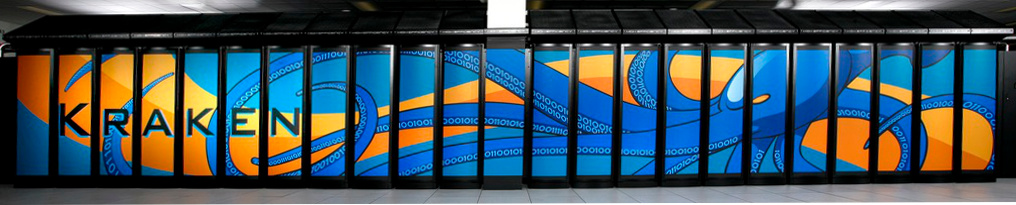
\includegraphics{../common/pics/krakenWide}
  \end{block}
\end{frame}

\begin{frame}[fragile]
  \begin{block}{Covariance Code}
    \begin{align*}
    cov(x_{n\times p}) = 
\frac{1}{n-1}\sum_{i=1}^n\left(x_i-\mu_x\right)\left(x_i-\mu_x\right)^T
  \end{align*}
\begin{lstlisting}
x <- ddmatrix("rnorm", nrow=n, ncol=p, mean=mean, sd=sd)

cov.x <- cov(x)
\end{lstlisting}
  \end{block}
\end{frame}

\begin{frame}
  \begin{block}{\code{cov()}}
  \begin{center}
    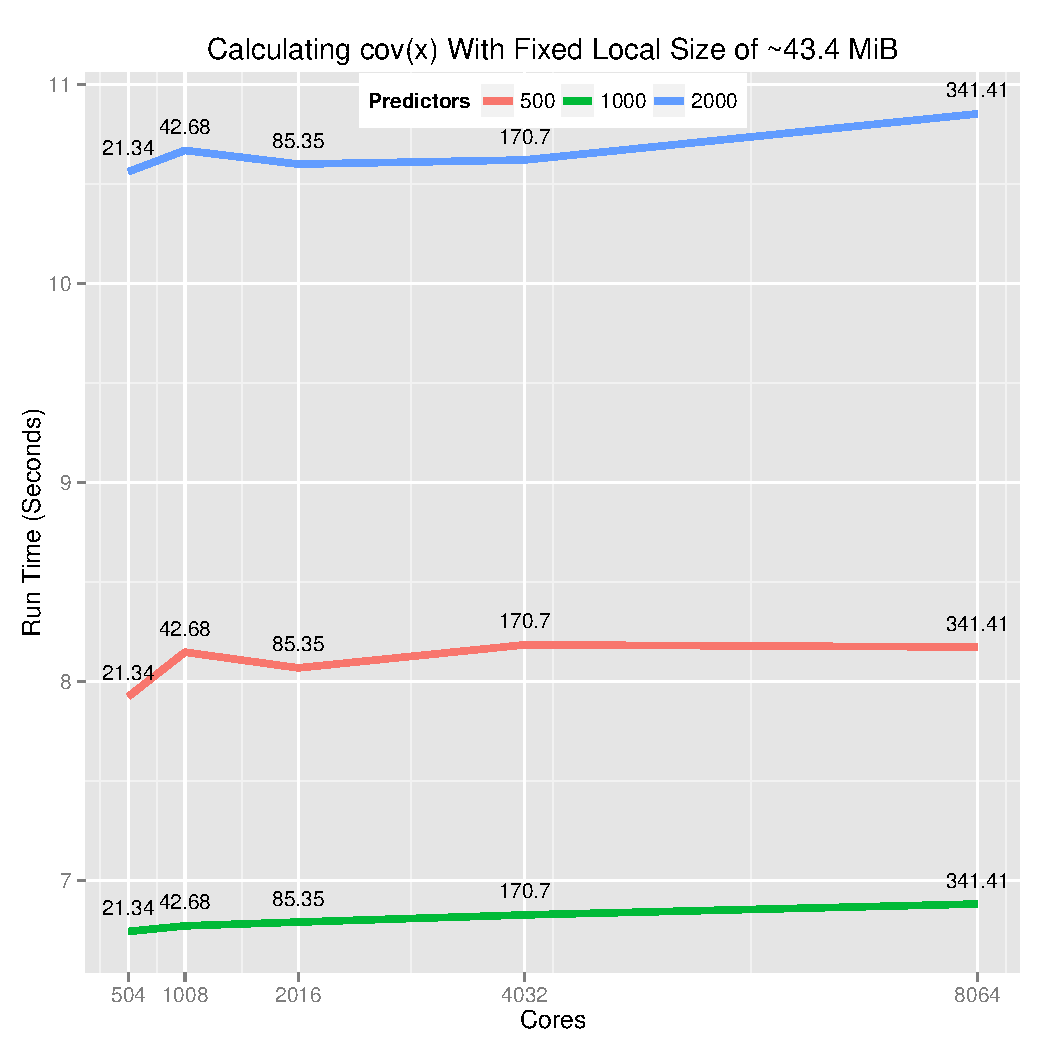
\includegraphics[height=.88\textheight]{../common/pics/cov}
  \end{center}
  \end{block}
\end{frame}

\begin{frame}[fragile]
  \begin{block}{Linear Model Code}
      Find $\bbeta$ such that
      \begin{align*}
      \by = \bX\bbeta + \bepsilon
      \end{align*}

      When $\bX$ is full rank,
      \begin{align*}
      \hat{\bbeta} = (\bX^T\bX)^{-1}\bX^T\by \label{math:ols}
      \end{align*}
\begin{lstlisting}
x <- ddmatrix("rnorm", nrow=n, ncol=p, mean=100, sd=10000)
beta_true <- ddmatrix("runif", nrow=p, ncol=1)

y <- x %*% beta_true

beta_est <- lm.fit(x, y)$coefficients
\end{lstlisting}  %$end
  \end{block}
\end{frame}

\begin{frame}
  \begin{block}{\code{lm.fit()}}
  \begin{center}
    \includegraphics[height=.88\textheight]{../common/pics/benchmarks/lmfit2}
  \end{center}
  \end{block}
\end{frame}

\begin{frame}
  \begin{block}{\code{Data Generation}}
  \begin{center}
    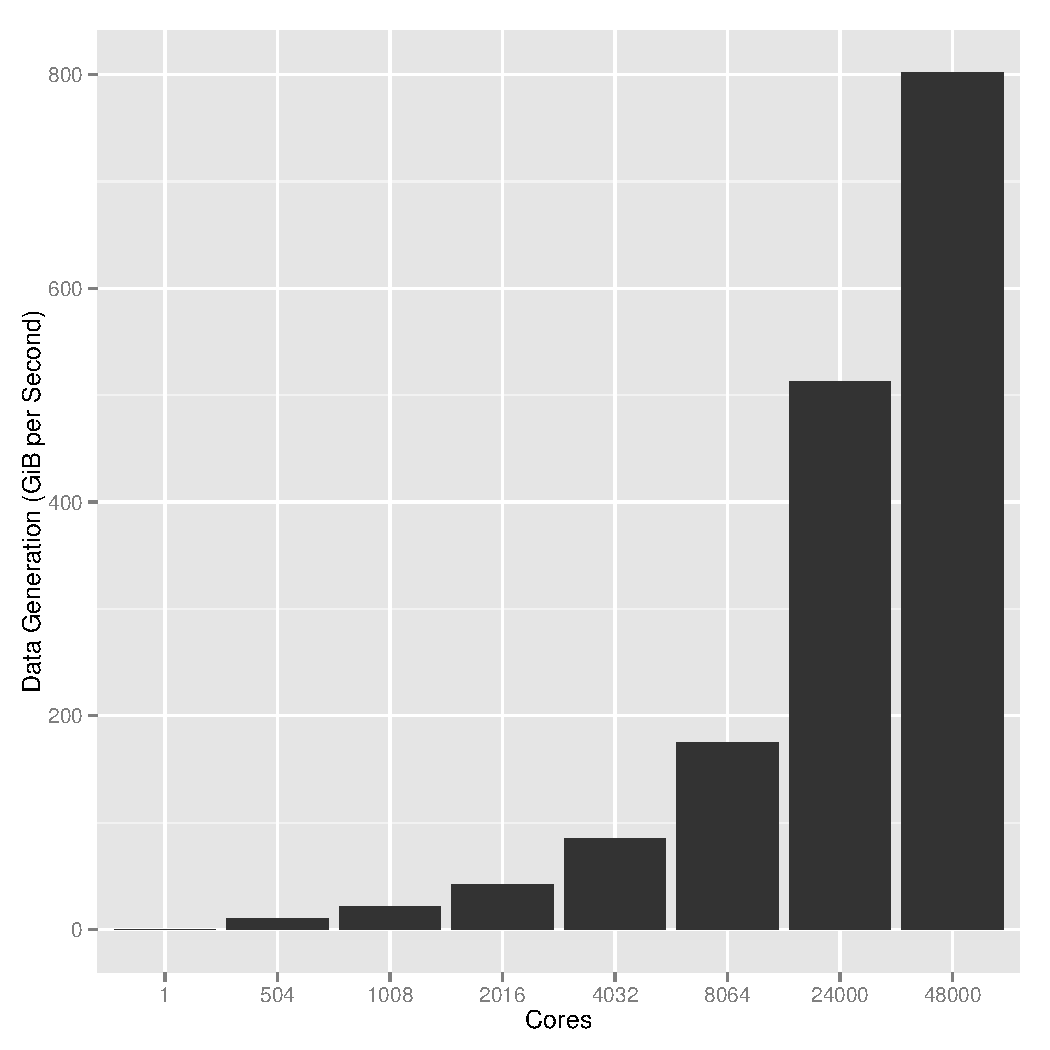
\includegraphics[height=.88\textheight]{../common/pics/benchmarks/datagen24k}
  \end{center}
  \end{block}
\end{frame}

\begin{frame}
  \begin{block}{PCA Benchmark Data}
    \begin{enumerate}[<+-|alert@+>]
      \item Measure wallclock time for principal components analysis
      \item Random normal $N(100, 10000)$
      \item Global problem size fixed
      \item ``strong scaling'' = local problem decreases with core count
      \item Two sets: 50,000 $\times$ 50,000 and 100,000 $\times$ 100,000
      \item Runs out of local work as core count increases
    \end{enumerate}
    \vspace{.8cm}
    \centering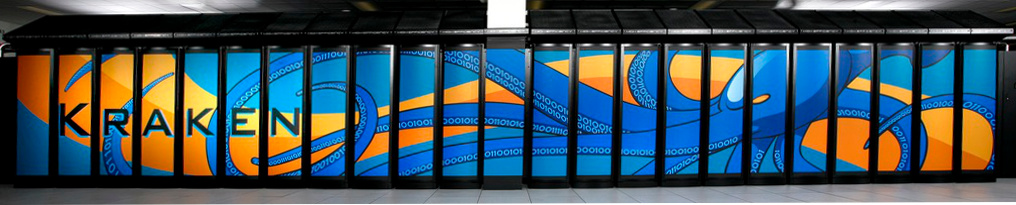
\includegraphics{../common/pics/krakenWide}
  \end{block}
\end{frame}

\begin{frame}
  \begin{block}{\code{prcomp() Strong Scaling}}
  \begin{center}
    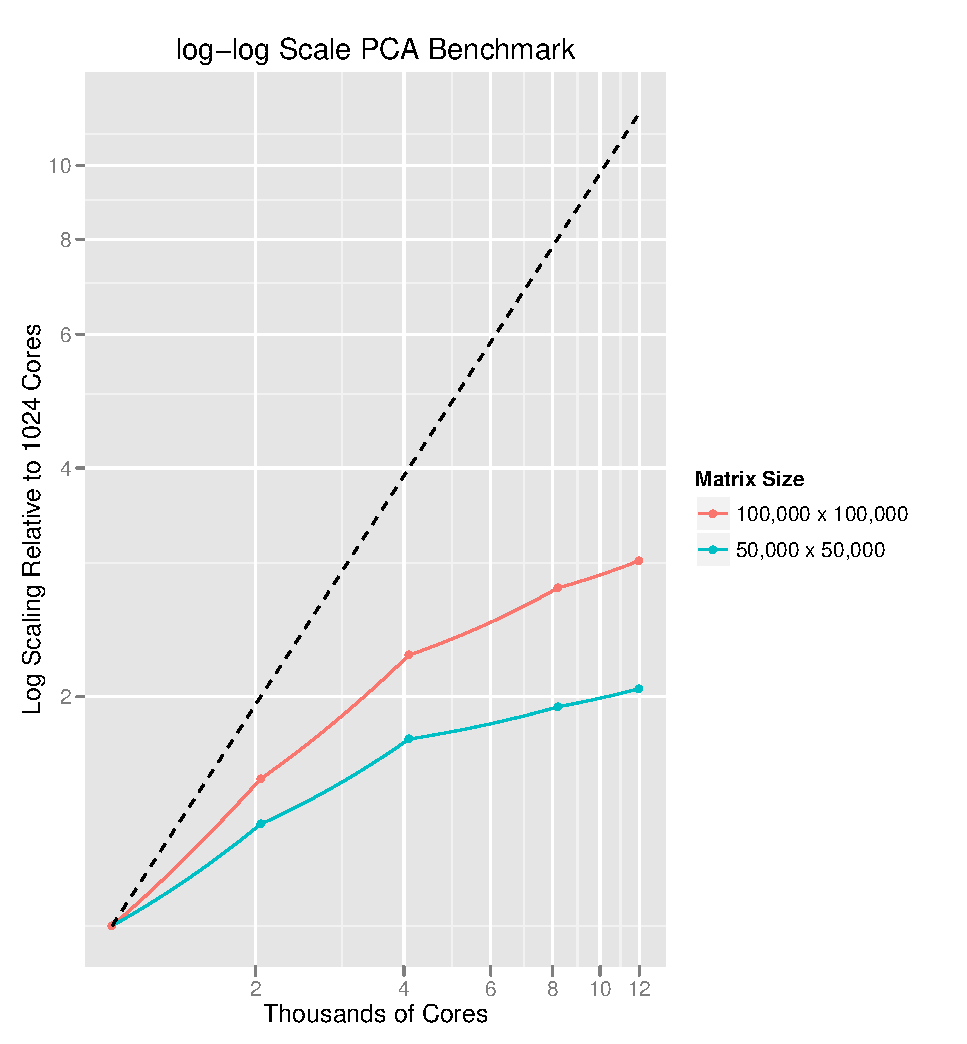
\includegraphics[height=.88\textheight]{../common/pics/benchmarks/pca_scaling}
  \end{center}
  \end{block}
\end{frame}
\section{Applications}
\makesubcontentsslides

\subsection{RandSVD}
\makesubcontentsslidessec


\begin{frame}[fragile]
\fontsize{8pt}{10}\selectfont
\begin{block}{Randomized truncated SVD\footnotemark}
  \begin{minipage}{.56\textwidth}
    \begin{center}
      \includegraphics[height=.41\textheight]{../common/pics/randsvd/randSVDalg}
      \\
      \includegraphics[height=.26\textheight]{../common/pics/randsvd/randSVDalg4_4}
    \end{center}
  \end{minipage}
%   \hspace{.01cm}
  \begin{minipage}{0.43\textwidth}
\begin{lstlisting}[title=Serial 
R,basicstyle=\tiny,backgroundcolor=\color{grayish} 
,numberstyle=\tiny\color{black},keywordstyle=\color{black},commentstyle=\color{ 
dkgreen},stringstyle=\color{black},escapeinside={(*@}{@*)}]
randSVD <- function(A, k, q=3)
  {
    ## Stage A
    Omega <- (*@ matrix(rnorm(n*2*k),@*)
      (*@ nrow=n, ncol=2*k) @*)
    Y <- A %*% Omega
    Q <- qr.Q(qr(Y))
    At <- t(A)
    for(i in 1:q)
      {
        Y <- At %*% Q
        Q <- qr.Q(qr(Y))
        Y <- A %*% Q
        Q <- qr.Q(qr(Y))
      }
    
    ## Stage B
    B <- t(Q) %*% A
    U <- La.svd(B)$u
    U <- Q %*% U
    U[, 1:k]
  }
\end{lstlisting} %balance$
\end{minipage}
{\fontsize{6pt}{10}\selectfont $^1$Halko, Martinsson, 
  and Tropp. 2011. Finding structure with randomness: probabilistic
  algorithms  for constructing \\[-1ex] approximate matrix decompositions
  \emph{SIAM Review} \textbf{53} 217--288}
\end{block}
\end{frame}


\begin{frame}[fragile]
 \fontsize{8pt}{10}\selectfont
\begin{block}{Randomized truncated SVD}
  \hfill
  \begin{minipage}{0.430\textwidth}
\begin{lstlisting}[title=Serial 
R,basicstyle=\tiny,backgroundcolor=\color{grayish} 
,numberstyle=\tiny\color{black},keywordstyle=\color{black},commentstyle=\color{ 
dkgreen},stringstyle=\color{black},escapeinside={(*@}{@*)}]
randSVD <- function(A, k, q=3)
  {
    ## Stage A
    Omega <- (*@ \textcolor{blue}{matrix(rnorm(n*2*k),} @*)
      (*@ \textcolor{blue}{ nrow=n, ncol=2*k)} @*)
    Y <- A %*% Omega
    Q <- qr.Q(qr(Y))
    At <- t(A)
    for(i in 1:q)
      {
        Y <- At %*% Q
        Q <- qr.Q(qr(Y))
        Y <- A %*% Q
        Q <- qr.Q(qr(Y))
      }
    
    ## Stage B
    B <- t(Q) %*% A
    U <- La.svd(B)$u
    U <- Q %*% U
    U[, 1:k]
  }
\end{lstlisting} %balance$
  \end{minipage}
  \hfill
  \begin{minipage}{0.430\textwidth}
\begin{lstlisting}[title=Parallel pbdR,basicstyle=\tiny,backgroundcolor=\color{
grayish}, numberstyle=\tiny\color{black},keywordstyle=\color{black},
commentstyle=\color{dkgreen},stringstyle=\color{black},escapeinside={(*@}{@*)}]
randSVD <- function(A, k, q=3)
  {
    ## Stage A
    Omega <- (*@ \textcolor{blue}{ddmatrix("rnorm",} @*)
      (*@ \textcolor{blue}{nrow=n, ncol=2*k)} @*)
    Y <- A %*% Omega
    Q <- qr.Q(qr(Y))
    At <- t(A)      
    for(i in 1:q)
      {
        Y <- At %*% Q   
        Q <- qr.Q(qr(Y))
        Y <- A %*% Q    
        Q <- qr.Q(qr(Y))
      }
    
    ## Stage B
    B <- t(Q) %*% A     
    U <- La.svd(B)$u 
    U <- Q %*% U     
    U[, 1:k]
  }
\end{lstlisting}  % balancing $
  \end{minipage}
\hfill
\end{block}
\end{frame}

\begin{frame}
  \begin{block}{From journal to scalable code and scaling data in one day.}
    \begin{center}
      \includegraphics[width=.4\textwidth]{../common/pics/randsvd/randSVDspeedup}
      \hspace{1cm}
      \includegraphics[width=.4\textwidth]{../common/pics/randsvd/randSpeedupSVD}
    \end{center}
  \end{block}
\end{frame}

\subsection{Precipitation Extremes in Climate Simulation Data}
\begin{frame}
  \begin{block}{\pkg{pmclust}: EM algorithm for Gaussian mixture
      model clustering}
    \begin{minipage}{6cm}\scriptsize
      \begin{itemize}
      \item High resolution (~25 km) atmospheric model, CAM 5.1
      \item Start with 2.9 TB, read and subset to extremes of 4 variables with
        256 cores
      \item Using multiple starts and Rand index, determine number of clusters
      \item Describes patterns of extreme precipitation across
        atmospheric layers of moisture, temperature, and wind velocity
      \end{itemize}
    \end{minipage}
    \begin{minipage}{5.8cm}
      \includegraphics[height=3.8cm]{pics/T_K_04_R_05}
      \includegraphics[height=3.8cm]{pics/Q_K_04_R_05}
      \includegraphics[height=3.8cm]{pics/OMEGA_K_04_R_05}
    \end{minipage}
    \vspace{-4.5ex}
    \begin{center}
      \includegraphics[trim=2mm 0mm 3mm 0mm,clip=true,height=3.4cm]{pics/tiles_4d_all_sort}
      \includegraphics[height=3cm]{pics/map_K_04_R_05}
      \includegraphics[trim=0mm 0mm 2mm 0mm,clip=true,height=3cm]{pics/PRECT_K_04_R_05}
    \end{center}
      \end{block}
\tiny Chen, Ostrouchov, Pugmire, Prabhat, and Wehner (2013). A
Parallel EM Algorithm for Model-Based Clustering \\[-2ex] Applied to the
Exploration of Large Spatio-Temporal Data. Technometrics {\bf 55}, p.513-523.
\end{frame}

\subsection{Ocean Turbulence Characterization}
\begin{frame}
  \begin{block}{Principal components analysis}
    \begin{itemize}\scriptsize
    \item Ocean turbulence data (2013 INCITE), 70GB per time step,
      interactive with 128 cores 
    \item Variability analysis quantifies organization into large
      coherent structures: for 99\% variability, 250 components needed at T=1
      but only 50 needed at T=30
    \end{itemize}
    \vspace{-3ex}
    \begin{center}
      \includegraphics[trim=.8cm 11.5cm 0.6cm 0cm,clip=true,height=3.8cm]{pics/TurbulencePCA}
    \end{center}
  \end{block}
  \begin{raggedright}\tiny
    Ostrouchov, Pugmire, Rosenberg, Chen, and Pouquet (2013)
    Computation and volume rendering of large-scale EOF \\[-2ex] coherent modes
    in rotating turbulent flow data, AGU Fall Meeting, December, 2013.
  \end{raggedright}
\end{frame}

\subsection{Biogeography models}

\begin{frame}
  \begin{block}{Biogeography matrix exponentiation}
    \begin{minipage}{5cm}
      \begin{itemize}\tiny
      \item Fitting biogeography models requires many matrix exponentiations
      \item Benchmark: Matrix exponential of 5000$\times$5000 matrix.
      \item R 3.1.0, Matrix 1.1-2, rexpokit 0.25, pbdDMAT 0.3-0
      \item Libs: Cray LibSci, NETLIB ScaLAPACK, Compilers: gnu 4.8.2
      \item Configuration: 1 thread == 1 MPI rank == 1 physical core
      \end{itemize}
      \vspace{-4ex}
      \begin{center}
        \includegraphics[trim=4cm 2cm 3.5cm 2.2cm,clip=true,height=4cm]{pics/Biogeography}
      \end{center}
    \end{minipage}
    \begin{minipage}{6.9cm}
      \includegraphics[trim=1mm 1mm 1mm 1mm,clip=true,height=7cm]{pics/MatExp}
    \end{minipage}
  \end{block}
  \begin{raggedright}\tiny
    Schmidt and Matzke (2014) Distributed matrix exponentiation, The R
    User Conference (UseR! 2014), \\[-2ex] Los Angeles, CA, August 2014 .
  \end{raggedright}
\end{frame}

\section{Challenges}

\hidenum
\begin{frame}[noframenumbering]
\frametitle{Contents}
 \tableofcontents[currentsection,hideallsubsections]
\end{frame}
\shownum


\subsection{Challenges}

\begin{frame}
  \begin{block}{Challenges}
    \begin{itemize}[<+-|alert@+>]
      \item Perceptions.
      \item Library loading.
      \item Profiling.
    \end{itemize}
  \end{block}
\end{frame}


\begin{frame}
  \begin{block}{Covariance Revisited: Distributed Data Parameter Calibration}
    \begin{center}
     \includegraphics[width=10cm, height=7cm]{../common/pics/cov_param}
    \end{center}
  \end{block}
\end{frame}

\begin{frame}
  \begin{block}{Adding More Levels of Parallelism}
    \begin{center}
      {\color{dkblue}Distributed Memory (cluster nodes)} \\
      {\color{dkgreen}Shared Memory (multicore)} \\
      {\color{purple}Co-Processor (GPU, manycore)}
    \end{center}
    \begin{itemize}
      \item {\color{dkblue}pbdDMAT} + {\color{purple}CUBLAS}: near term on Titan 
      \item {\color{dkblue}pbdDMAT} - {\color{dkblue}ScaLAPACK} +
        {\color{dkblue}D}{\color{dkgreen}PLASMA}: QR only 
      \item {\color{dkblue}pbdDMAT} + {\color{dkgreen}PLASMA} or
        {\color{dkgreen}MKL} or {\color{dkgreen}ACML}: often helps 
      \item {\color{dkblue}pbdDMAT} + {\color{purple}MAGMA}: may not help 
    \end{itemize}
  \end{block}
\end{frame}

\hidenum
\section*{}
\begin{frame}[noframenumbering]
  \begin{block}{Tutorials}
  \begin{itemize}
    \item {\small OLCF Very Large Data Workshop
         ... {\color{red} NEXT!}}
    \item {\small Seoul National University, August 20}
    \item {\small SC13, November 17-22, Denver}
  \end{itemize}
  \end{block}
  \begin{block}{Invited Talks}
  \begin{itemize}
    \item {\small International Association for Statistical Computing, Aug 22-23, Seoul}
    \item {\small 59th ISI World Statistics Congress, August 25-30, Hong Kong }
  \end{itemize}
  \end{block}
\end{frame}
  
\begin{frame}[noframenumbering]
 \begin{block}{Thanks for coming!}
 \begin{center}
     {\Large Questions?}\\[1cm]
     {\Large Be sure to stick around for the tutorial!}
  \end{center}
 \end{block}
\end{frame}

\section{Getting Started}
\makesubcontentsslides


% \begin{frame}[fragile,shrink]
%   \begin{block}{Embarrassingly Parallel Computation}\pause
%     \vspace{-1ex}
%     \begin{minipage}[t]{.45\textwidth}
%       \begin{lstlisting}[title=EPforeach.R "asking for parallel",basicstyle=\tiny]
% library(doMPI, quiet=TRUE)
% cl <- startMPIcluster()
% registerDoMPI(cl)

% n <- 10
% myIn <- vector("list", n)

% myFun <- function(x) {
%   s <- sum(rnorm(10000))
%   rank <- mpi.comm.rank(comm=0)
%   return(paste(s, "from", rank))
% }

% results <- foreach(i = 1:n) %dopar% {
%   out <- myFun(myIn[[i]])
% }

% print(results)

% closeCluster(cl)
% mpi.quit()
%       \end{lstlisting}
%     \end{minipage}
%     \hfill
%     \begin{minipage}[t]{.5\textwidth}
%       \begin{lstlisting}[title=EPpbdR.R "thinking parallel",basicstyle=\tiny]
% library(pbdMPI, quiet=TRUE)
% init()

% myChunk <- get.jid(n <- 10)
% myIn <- vector("list", length(myChunk))
% myOut <- vector("list", length(myChunk))

% myFun = function(x) {
%   s <- sum(rnorm(10000))
%   rank <- comm.rank()
%   return(paste(s, "from", rank))
% }

% for(i in 1:length(myChunk)) {
%   myOut[[i]] <- myFun(myIn[[i]])
% }
% results <- unlist(gather(myOut), recursive=FALSE)

% comm.print(results)
% finalize()
%       \end{lstlisting}
%     \end{minipage}
%   \end{block}
% \end{frame}



% \begin{frame}[fragile,shrink]
%   \begin{block}{ddmatrix Computation}\pause
%     \vspace{-1ex}
%     \begin{lstlisting}[title=pbdRddmatrix.R "being parallel",basicstyle=\tiny]
% library(pbdDMAT, quiet=TRUE)
% init.grid()

% x <- ddmatrix(1:70, nrow=10, ncol=7)
% comm.print(x@Data, all.rank=TRUE)
% y <- as.rowblock(x)
% comm.print(y@Data, all.rank=TRUE)

% cx <- t(x) %*% x
% cx2 <- crossprod(x)

% all.equal(cx, cx2)

% comm.print(cx@Data, all.rank=TRUE)

% x.pca <- prcomp(x)

% comm.print(x.pca)
% comm.print(names(x.pca))
% comm.print(x.pca$rotation)
% comm.print(x.pca$rotation@Data, all.rank=TRUE)

% finalize()
%     \end{lstlisting}
%   \end{block}
% \end{frame}



\end{document}